\documentclass[12pt,aspectratio=169]{beamer}

% ====================================================
% ====================================================
% USEPACKAGES AND IMPORTS
% ====================================================
% ====================================================

\usepackage[T1]{fontenc}
\usepackage[utf8]{inputenc}
\usepackage[english]{babel}

% tables
\usepackage{tabularx}
\usepackage{colortbl}
\usepackage{multirow}
\usepackage{makecell}

% tikz and colors
\usepackage{tikz}
\usepackage{xcolor}
\usepackage{pgfplots}
\usepackage{pgfplotstable}
\usepackage{tikzsymbols}

\usetikzlibrary{calc}
\usetikzlibrary{trees}
\usetikzlibrary{patterns}
\usetikzlibrary{shadings}
\usetikzlibrary{positioning}
\usetikzlibrary{intersections}
\usepgfplotslibrary{patchplots}
\usepgfplotslibrary{fillbetween}
\usetikzlibrary{decorations.pathreplacing}

\usetikzlibrary{arrows}
\usetikzlibrary{arrows.meta}

\usetikzlibrary{shapes}
\usetikzlibrary{shapes.arrows}
\usetikzlibrary{shapes.callouts}
\usetikzlibrary{shapes.symbols}
\usetikzlibrary{shapes.geometric}

% boxes
\usepackage[many]{tcolorbox}

% math packages and fonts
\usepackage{bm}
\usepackage{ccfonts}
\usepackage{eulervm}
\usepackage{amsmath}
\usepackage{amsfonts}
\usepackage{amssymb}
\usepackage{amsthm}
\usepackage{mathtools}
\usepackage{nicefrac}
\usepackage{slashed}
\usepackage{bbold}
\usepackage{array}
\usepackage{cancel}

% algorithms and listings
\usepackage[ruled,vlined,linesnumbered]{algorithm2e}
\usepackage{listings}
\usepackage{setspace}

\tcbuselibrary{listings}
\tcbuselibrary{breakable}
\tcbuselibrary{skins}

% misc
\usepackage{soul}
\usepackage{pifont}
\usepackage{skull}
\usepackage{multicol}
\usepackage{animate}
\usepackage{hyperref}
\usepackage{wasysym}
\usepackage[absolute,overlay]{textpos}
\usepackage[hang,flushmargin]{footmisc}

% ====================================================
% ====================================================
% LAYOUT AND THEME
% ====================================================
% ====================================================

\usetheme{Copenhagen}

% color definitions
\definecolor{myblue1}{RGB}{35,119,189}
\definecolor{myblue2}{RGB}{95,179,238}
\definecolor{myblue3}{RGB}{129,168,207}
\definecolor{myblue4}{RGB}{26,89,142}

\definecolor{myred1}{RGB}{247,12,12}

% set theme colors
\setbeamercolor*{structure}{fg=myblue1,bg=blue}
\setbeamercolor*{palette primary}{use=structure,fg=white,bg=structure.fg}
\setbeamercolor*{palette secondary}{use=structure,fg=white,bg=structure.fg!75!black}
\setbeamercolor*{palette tertiary}{use=structure,fg=white,bg=structure.fg!50!black}
\setbeamercolor*{palette quaternary}{fg=black,bg=white}

\setbeamertemplate{itemize item}[circle]
\setbeamertemplate{itemize subitem}[circle]
\setbeamertemplate{itemize subsubitem}[circle]

\setbeamertemplate{enumerate item}[circle]
\setbeamertemplate{enumerate subitem}[circle]
\setbeamertemplate{enumerate subsubitem}[circle]

\setbeamercolor{itemize item}{fg=myblue1}
\setbeamercolor{itemize subitem}{fg=myblue1}
\setbeamercolor{itemize subsubitem}{fg=myblue1}

\setbeamertemplate{section in toc}[circle]
\setbeamertemplate{subsection in toc}[circle]
\setbeamerfont{subsection in toc}{size=\scriptsize}

\setbeamercolor{frametitle continuation}{fg=black}

% title graphic -- sap logo and dhbw logo
\titlegraphic{
\includegraphics[scale=0.1]{../03_img/logo_sap}\hspace*{4.75cm}~%
   	
\includegraphics[scale=0.05]{../03_img/logo_dhbw}
}

\makeatletter
% frame title
\defbeamertemplate*{frametitle}{mydefault}[1][left]
{
  	\ifbeamercolorempty[bg]{frametitle}{}{\nointerlineskip}%
  	\nointerlineskip%
 	\@tempdima=\textwidth%
  	\advance\@tempdima by\beamer@leftmargin%
  	\advance\@tempdima by\beamer@rightmargin%
  	\begin{tcolorbox}[
  		enhanced,
  		outer arc=0pt,
  		arc=0pt,
  		boxrule=0pt,
  		top=0pt,
  		bottom=0pt,
  		enlarge left by=-\beamer@leftmargin,
  		enlarge right by=-\beamer@rightmargin,
  		width=\paperwidth,
  		nobeforeafter,
  		interior style={
    			left color=myblue2,
    			right color=white
    		},
  		shadow={0mm}{-0.4mm}{0mm}{black!60,opacity=0.6},    
  		shadow={0mm}{-0.8mm}{0mm}{black!40,opacity=0.4},    
  	]
    	\usebeamerfont{frametitle}%
    	\vbox{}\vskip-1ex%
    	\if@tempswa\else\csname beamer@fte#1\endcsname\fi%
    	\insertframetitle\par%
    	{%
      		\ifx\insertframesubtitle\@empty%
      		\else%
      		{\usebeamerfont{framesubtitle}\usebeamercolor[fg]{black}\insertframesubtitle\strut\par}%
      		\fi
    	}%
    	\vskip-1ex%
    	\if@tempswa\else\vskip-.3cm\fi
  	\end{tcolorbox}%
}

% footline of a frame
\defbeamertemplate*{footline}{mysplit theme}
{%
  	\leavevmode%
  	\hbox{
		\begin{beamercolorbox}[
			wd=.5\paperwidth,ht=2.5ex,dp=1.125ex,leftskip=.3cm plus1fill,rightskip=.3cm
		]{author in head/foot}%
    			\usebeamerfont{author in head/foot}\insertshortauthor\ (\insertinstitute), \insertdate
  		\end{beamercolorbox}%
  		\begin{beamercolorbox}[
			wd=.5\paperwidth,ht=2.5ex,dp=1.125ex,leftskip=.3cm,rightskip=.3cm plus1fil
		]{title in head/foot}%
    			\usebeamerfont{title in head/foot}\insertshorttitle\hfill
    			\insertprefix-\insertframenumber/\inserttotalframenumber\hspace*{0.5em}
  		\end{beamercolorbox}}%
  	\vskip0pt%
}
\makeatother

% ====================================================
% ====================================================
% COMMANDS AND GENERAL DEFINITIONS
% ====================================================
% ====================================================

% page number prefix
\newcommand\insertprefix{}  % empty by default
\newcommand\prefix[1]{\renewcommand\insertprefix{#1}}

% math definitions
% ====================================================
\DeclareMathOperator*{\argmax}{arg\,max}
\DeclareMathOperator*{\argmin}{arg\,min}
\newcommand*\diff{\mathop{}\!\mathrm{d}}

\newcommand*{\vertbar}{\rule[-1ex]{0.5pt}{2.5ex}}
\newcommand*{\horzbar}{\rule[.5ex]{2.5ex}{0.5pt}}

% commands
% ====================================================

% highlight commands
% --------------------------------------------------------------------------------------------------------
% highlight command
\newcommand{\highlight}[1]{\textcolor{myblue1}{\textbf{#1}}}
\newcommand{\highlighttt}[1]{\textcolor{myblue1}{\texttt{#1}}}
\newcommand{\Highlight}[1]{\textcolor{myred1}{\textbf{#1}}}

% blue color boxes (with frame/without frame/without fill)
\newtcolorbox{boxBlue}{colback=myblue1!10!white,colframe=myblue4}
\newtcolorbox{boxBlueNoFrame}{colback=myblue1!10!white,colframe=myblue1!10!white}
\newtcolorbox{boxBlueNoFill}{colback=white,colframe=myblue4}

% font commands
% --------------------------------------------------------------------------------------------------------
\newcommand{\linkstyle}[1]{\underline{\smash{\texttt{#1}}}} 		% style of hyperlinks

% tikz commands
% --------------------------------------------------------------------------------------------------------

% yellow sticky note
\newcommand{\bubble}[3]{
\begin{textblock}{100}(#1, #2)
      	\begin{tikzpicture}
		\node[rectangle,draw=yellow,very thick,fill=yellow!60,align=center] at (0,0) {#3};
	\end{tikzpicture}
\end{textblock}
}

\newcommand{\floattext}[3]{
\begin{textblock}{100}(#1, #2)
      	#3
\end{textblock}
}

\newcommand{\doublecircle}[2]{
	\draw[fill=white,draw=myblue1] (#1,#2) circle (2mm);
	\draw[fill=myblue1,draw=myblue1] (#1,#2) circle (1.5mm);
}

% slide modifiers
% --------------------------------------------------------------------------------------------------------
% mark slide as optional
\newcommand{\optional}{
	\begin{textblock}{100}(0.15,0.30)
      		
\includegraphics[scale=0.2]{../03_img/scream}
    	\end{textblock}
}

% mark slide as important
\newcommand{\important}{
	\begin{textblock}{100}(0.10,0.15)
      		
\includegraphics[scale=0.1]{../03_img/important}
    	\end{textblock}
}

% citation
% --------------------------------------------------------------------------------------------------------
% first argument in {book, online, article}
\newcommand{\literature}[5]{
	\setbeamertemplate{bibliography item}[#1]
	\bibitem{#2}
	\highlight{#3} \\
	\textcolor{darkgray}{\textit{#4}} \\
	\textcolor{black}{#5}
}
% cite content
\newcommand{\citeAuthor}[3]{\vfill\scriptsize\textcolor{lightgray}{#1 \cite{#2} #3}}

% slide architecture
% --------------------------------------------------------------------------------------------------------
% divide frame into two parts
\newcommand{\divideTwo}[4]{
	\begin{minipage}{#1\textwidth}
		#2
	\end{minipage}
	\hfill
	\begin{minipage}{#3\textwidth}
		#4
	\end{minipage}
}

% divide frame into two parts (start on top)
\newcommand{\divideTwoTop}[4]{
	\begin{minipage}[t]{#1\textwidth}
		#2
	\end{minipage}
	\hfill
	\begin{minipage}[t]{#3\textwidth}
		#4
	\end{minipage}
}

% special pages
% --------------------------------------------------------------------------------------------------------
% title page
\newcommand{\maketitlepage}{
	{
		\beamertemplatenavigationsymbolsempty
		\usebackgroundtemplate{%
			\tikz[overlay,remember picture] \node[opacity=0.2, at=(current page.center)] {
  				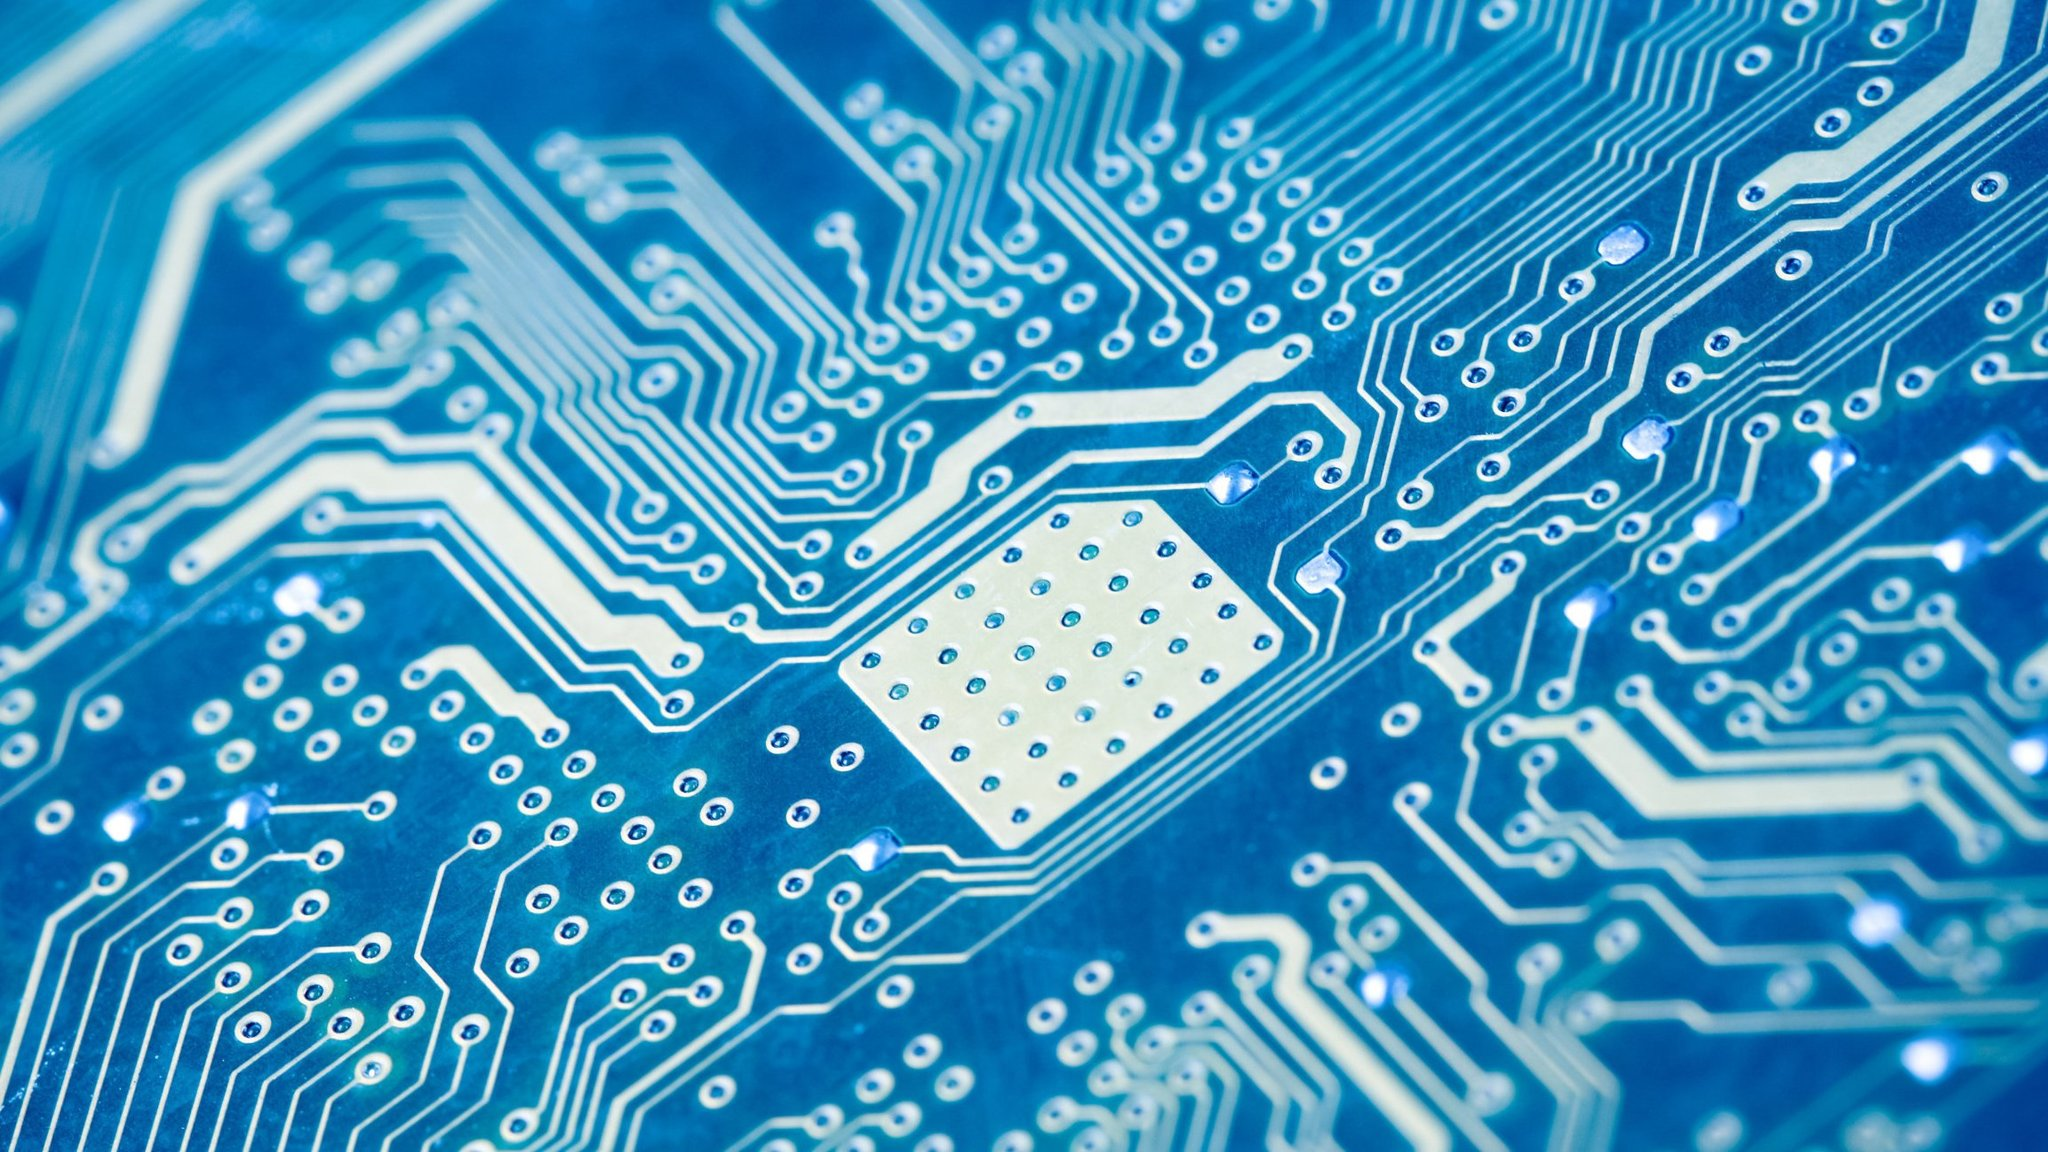
\includegraphics[height=\paperheight,width=\paperwidth]{../03_img/processor.jpg}
			};
		}
		\begin{frame}[plain]
			\vspace*{0.75cm}
			\maketitle
			\vfill
			\begin{center}
				\footnotesize Find all slides on \href{https://github.com/DaWe1992/Applied_ML_Fundamentals}{\linkstyle{GitHub}}
			\end{center}
		\end{frame}
	}
}

% divider page
\newcommand{\makedivider}[1]{
	{
		\beamertemplatenavigationsymbolsempty
		\usebackgroundtemplate{%
			\tikz[overlay,remember picture] \node[opacity=0.2, at=(current page.center)] {
  				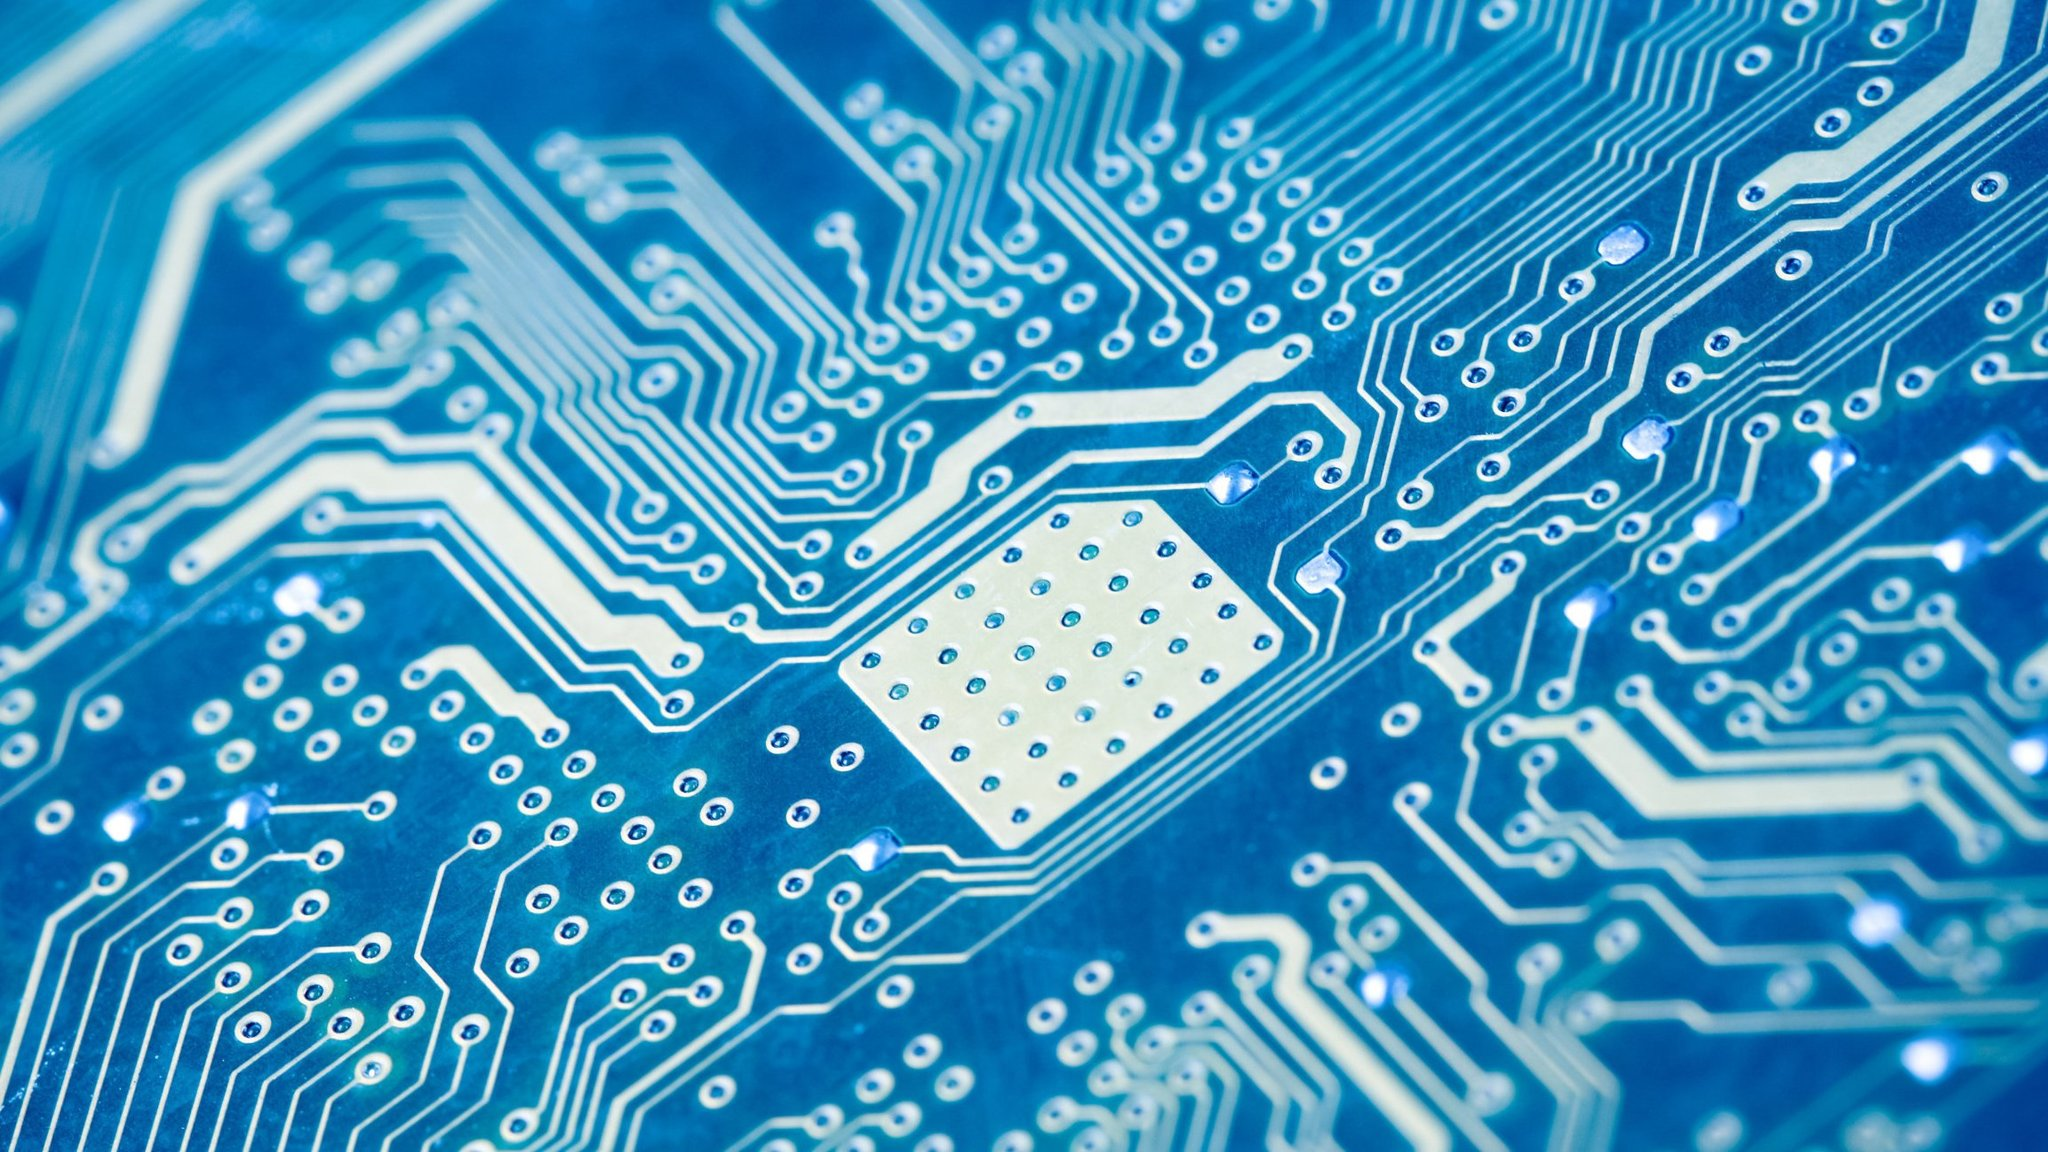
\includegraphics[height=\paperheight,width=\paperwidth]{../03_img/processor.jpg}
			};
		}
		\begin{frame}[plain]
			\vfill
			\begin{boxBlue}
				\centering
				\textbf{Section:} \\
				\large \highlight{#1}
			\end{boxBlue}
			\vfill
			\centering
			
\includegraphics[scale=0.05]{../03_img/logo_dhbw.png}
			\vfill
		\end{frame}
	}
}

% overview page
\newcommand{\makeoverview}[1]{
	\begin{frame}{Lecture Overview}{}
		\begin{tabbing}
			\hspace*{3.5cm}\= \kill
			\ifnum #1=1 \highlight{\textbf{Unit I:}} \else \textbf{Unit I:} \fi
			\> \ifnum #1=1 \highlight{Machine Learning Introduction} \else Machine Learning Introduction \fi \\
		\end{tabbing}
	\end{frame}
}

% thank you page
\newcommand{\makethanks}{
	{\beamertemplatenavigationsymbolsempty
	\begin{frame}[plain]
		\vfill
		\begin{boxBlue}
			\centering
			\Large \highlight{Thank you very much for the attention!}
		\end{boxBlue}
		
		\vfill\footnotesize
		\begin{tabbing}
			\hspace*{1.5cm}\= \kill
			\highlight{Topic:} 	\> \inserttitle \\
			\highlight{Date:} 	\> \insertdate
		\end{tabbing}
		
		\vfill
		\highlight{Contact:} \\
		\insertauthor\ (D062271) \\
		\insertinstitute \\
		\href{mailto:daniel.wehner@sap.com}{\linkstyle{daniel.wehner@sap.com}}
		
		\vfill\normalsize
		\begin{center}
			\large\highlight{Do you have any questions?}
		\end{center}
		\vfill
	\end{frame}}
}

% global pfgplots settings
% --------------------------------------------------------------------------------------------------------
\pgfplotsset{
	% allow filtering of data for pgfplots
	discard if/.style 2 args={
        		x filter/.code={
            		\edef\tempa{\thisrow{#1}}
            		\edef\tempb{#2}
            		\ifx\tempa\tempb
                		\def\pgfmathresult{inf}
            		\fi
        		}
    	},
    	discard if not/.style 2 args={
        		x filter/.code={
            		\edef\tempa{\thisrow{#1}}
            		\edef\tempb{#2}
            		\ifx\tempa\tempb
            		\else
                		\def\pgfmathresult{inf}
            		\fi
        		}
    	}
}


% ====================================================
% ====================================================
% PRESENTATION DATA
% ====================================================
% ====================================================

\title[Reinforcement Learning]{*** Applied Machine Learning Fundamentals *** Reinforcement Learning}
\institute{SAP\,SE}
\author{M.\,Sc. Daniel Wehner}
\date{Winter term 2019/2020}
\prefix{RL}

% ====================================================
% ====================================================
% BEGIN OF DOCUMENT
% ====================================================
% ====================================================

\begin{document}

% Title frame
%______________________________________________________________________
\maketitlepage


% Lecture Overview
%______________________________________________________________________
%\begin{frame}{Lecture Overview}{}
%	\begin{center}
%		\Huge\highlight{Out of scope for this lecture!}
%	\end{center}
%\end{frame}


% Agenda
%______________________________________________________________________
\begin{frame}{Agenda for this Unit}
	\begin{multicols}{2}
		\tableofcontents
	\end{multicols}
\end{frame}


% Section: Introduction
%______________________________________________________________________
\section{Introduction}
\makedivider{Introduction}

% Subsection: Psychological Motivation
% --------------------------------------------------------------------------------------------------------
\subsection{Psychological Motivation}

% Psychological Motivation
\begin{frame}{Psychological Motivation}{}
	\divideTwo{0.69}{
		\begin{itemize}
			\item B. F. Skinner (1904 -- 1990)
			\item \highlight{Operant conditioning} (behaviorism)
			\begin{itemize}
				\item Associative learning
				\item Strength of a behavior is modified by reinforcement or punishment
				\item Operant behavior is \textbf{voluntary}
			\end{itemize}
			\item The image on the right depicts the `Skinner box'
		\end{itemize}
	}{0.29}{
		\begin{figure}
			\centering
			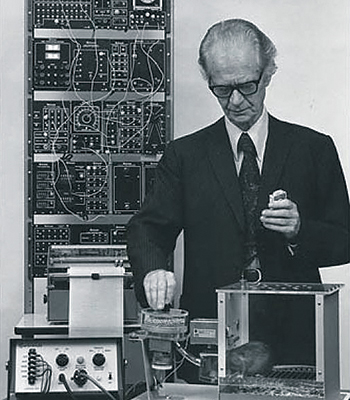
\includegraphics[scale=0.35]{14_rl/02_img/skinner_box}
		\end{figure}
	}
\end{frame}


% Psychological Motivation (Ctd.)
\begin{frame}{Psychological Motivation (Ctd.)}{}
	\begin{table}[h]
	\scalebox{0.8}{
		\renewcommand{\arraystretch}{1.75}
		\begin{tabularx}{15cm}{| Y | Y | Y |}
			\hline
			\textbf{Operant conditioning}			&
			\textbf{\textcolor{violet}{Punishment}}		&
			\textbf{\textcolor{orange}{Reinforcement}}	\\ \hline
			\textbf{\textcolor{green!70!black}{Positive}}	&	\textcolor{green!70!black}{add} noxious stimulus to \textcolor{violet}{decrease} behavior 	& 	\textcolor{green!70!black}{add} pleasant stimulus to \textcolor{orange}{increase} behavior 	\\ \hline
			\textbf{\textcolor{red}{Negative}} 		&	\textcolor{red}{remove} pleasant stimulus to \textcolor{violet}{decrease} behavior 		& 	\textcolor{red}{remove} noxious stimulus to \textcolor{orange}{increase} behavior 		\\ \hline
		\end{tabularx}
	}
\end{table}














\end{frame}


% Subsection: What is Reinforcement Learning?
% --------------------------------------------------------------------------------------------------------
\subsection{What is Reinforcement Learning?}

% What is Reinforcement Learning?
\begin{frame}{What is Reinforcement Learning?}{}
	\begin{itemize}
		\item Agent $\Leftrightarrow$ (Unknown) Environment
		\item \textbf{Goal}
		\begin{itemize}
			\item Learn optimal decisions based on feedback provided by the environment
			\item Environment rewards agent for actions but \highlight{does not (!)} reveal the correct solution
				(reward can be positive or negative)
		\end{itemize}
		\item \textbf{Applications}
		\begin{itemize}
			\item Games, e.\,g.:
			\begin{itemize}
				\item Tic-Tac-Toe: MENACE [\textit{Michie}, 1963]
				\item Backgammon: TD-Gammon [\textit{Tesauro}, 1995]
			\end{itemize}
			\item Other: E.\,g. 
				\href{https://www.youtube.com/watch?v=W_gxLKSsSIE}{\linkstyle{robot control}}
				\scriptsize (btw.: $robot_{en}$ derived from $robota_{cz}$ -- labor service)
		\end{itemize}
	\end{itemize}
\end{frame}


% Reward Hypothesis
\begin{frame}{Reward Hypothesis}{}
	\begin{itemize}
		\item All goals of an agent can be explained by a single scalar called the reward
		\item It is the RL practitioners' task to find the right set of rewards
		\item This is referred to as \highlight{reward shaping}
	\end{itemize}

	\vspace*{3mm}
	\begin{boxBlueNoFrame}
		\highlight{Reward hypothesis:} \\[2mm]
		\footnotesize
		\highlight{What we mean by goals and purposes can be well thought of as the maximization of the expected value of the cumulative sum of a received scalar signal (called reward).}
	\end{boxBlueNoFrame}
\end{frame}


% Dimensions of Learning: Type of Training Information
\begin{frame}{Dimensions of Learning: Type of Training Information}{}
	\begin{figure}
	\centering
	\begin{tikzpicture}[
		scale=0.5,
		every node/.style={scale=0.8},
		arrow/.style={
			shorten >=0.2cm,
			shorten <=0.2cm,
			->,
			thick
		}
	]
	
		\node[draw=black,thick,align=left] (A) at (0,4) {
			\textbf{Supervised Learning} \\
			$\bullet$ A `teacher' provides gold labels \\
			$\bullet$ Neural networks, decision trees, regression
		};

		\node[draw=myblue1,thick,align=left] (B) at (-5,0) {
			\highlight{Reinforcement Learning} \\
			$\bullet$ Feedback only \\
			$\bullet$ No labels
		};

		\node[draw=black,thick,align=left] (C) at (5,0) {
			\textbf{Semi-Supervised Learning} \\
			$\bullet$ Partly labeled data
		};

		\node[draw=black,thick,align=left] (D) at (0,-4) {
			\textbf{Unsupervised Learning} \\
			$\bullet$ No labels available \\
			$\bullet$ Clustering, Apriori, ...
		};
	
		\draw[arrow] (A) -- (B);
		\draw[arrow] (A) -- (C);
		\draw[arrow] (B) -- (D);
		\draw[arrow] (C) -- (D);

	\end{tikzpicture}
\end{figure}
\end{frame}


% Differences to other Approaches
\begin{frame}{Difference to other Approaches}{}
	\begin{enumerate}
		\item \textbf{Delayed rewards}
		\begin{itemize}
			\item Sequence of actions $\Rightarrow$ Problem of \highlight{temporal credit assignment}
			\item Which actions were good? Which were bad?
		\end{itemize}
		\item \textbf{Exploitation vs. exploration}
		\begin{itemize}
			\item Should the agent perform actions which are known to be good...
			\item ...or should it try out new (possibly even better) actions?
		\end{itemize}
		\item \textbf{Partially observable states} (not everything my be observable)
		\item \textbf{Life-long learning} 
		\begin{itemize}
			\item Environment may not be static, it could change!
			\item Agents need to adapt to these changes...
		\end{itemize}
	\end{enumerate}
\end{frame}


% Credit Assignment Problem
\begin{frame}{Credit Assignment Problem}{}
	\begin{itemize}
		\item \textbf{Fundamental problem in reinforcement learning}
		\begin{itemize}
			\item Especially in games: Reward at the end of the match (have I won or lost?)
			\item Central Question: \textbf{Which moves contributed to winning / losing?}
			\item This problem is referred to as the \highlight{credit assignment problem}
		\end{itemize}
		\item \textbf{Solution:}
		\begin{itemize}
			\item All moves of the sequence are rewarded / punished equally
			\item After many games the algorithm converges (bad moves will be reinforced less positively, good moves will be positively reinforced more often)
		\end{itemize}
	\end{itemize}
\end{frame}


% Subsection: MENACE (Matchbox Educable Noughts and Crosses Engine)
% --------------------------------------------------------------------------------------------------------
\subsection{MENACE (Matchbox Educable Noughts and Crosses Engine)}

% MENACE: Learning to play Tic-Tac-Toe
\begin{frame}{MENACE: Learning to play `Tic-Tac-Toe'}{}
	\divideTwo{0.49}{
		\begin{itemize}
			\item Introduced by [\textit{Mitchie}, 1963]
			\item Learns to play `Tic-Tac-Toe'
			\item MENACE stands for:
			{\fontfamily{pcr}\selectfont
			\begin{itemize}
				\item[] \highlight{M}atchbox
				\item[] \highlight{E}ducable
				\item[] \highlight{N}oughts
				\item[] \highlight{A}nd
				\item[] \highlight{C}rosses
				\item[] \highlight{E}ngine
			\end{itemize}}
		\end{itemize}
	}{0.49}{
		\vspace*{2mm}
		\begin{figure}
	\centering
	\begin{tikzpicture}[scale=0.4]
	
		\draw[thick] (-6,2) -- (6,2);
		\draw[thick] (-6,-2) -- (6,-2);
		\draw[thick] (-2,-6) -- (-2,6);
		\draw[thick] (2,-6) -- (2,6);
		\draw[very thick] (-6,-6) -- (-6,6) -- (6,6) -- (6,-6) -- cycle;

		\node at (0,0) {\Huge{\textcolor{blue}{$\bm{\times}$}}};
		\node at (0,4) {\Huge{\textcolor{blue}{$\bm{\times}$}}};
		\node at (-4,4) {\huge{\textcolor{red}{$\bm{\bigcirc}$}}};
		\node at (4,4) {\huge{\textcolor{red}{$\bm{\bigcirc}$}}};

	\end{tikzpicture}
\end{figure}
	}
\end{frame}


% MENACE: Setup
\begin{frame}{MENACE: Setup}{}
	\begin{itemize}
		\item \textbf{`Hardware':}
		\begin{itemize}
			\item 287 matchboxes (1 per playing position)
			\item Marbles in nine different colors (one color per field)
			\item Initially, each matchbox contains the same amount of marbles of each color
		\end{itemize}
		\item \textbf{Algorithm:}
		\begin{itemize}
			\item Choose matchbox corresponding to current playing position
			\item Pick a marble randomly from the matchbox
			\item Put marker (\textcolor{blue}{$\bm{\times}$} or \textcolor{red}{$\bm{\bigcirc}$})
				on the field that corresponds to the color
		\end{itemize}
		\item \highlight{How can good moves be reinforced positively?}
	\end{itemize}
\end{frame}


% MENACE: Visualized
\begin{frame}{MENACE: Visualized}{}
	\begin{figure}
	\centering
	\begin{tikzpicture}[scale=1.0]
	
		\node (A) at (-4,4) {
			\begin{tikzpicture}[scale=0.15]
				\draw[thick] (-6,2) -- (6,2);
				\draw[thick] (-6,-2) -- (6,-2);
				\draw[thick] (-2,-6) -- (-2,6);
				\draw[thick] (2,-6) -- (2,6);
				\draw[very thick] (-6,-6) -- (-6,6) -- (6,6) -- (6,-6) -- cycle;

				\node at (0,0) {\textcolor{blue}{$\bm{\times}$}};
				\node at (0,4) {\textcolor{blue}{$\bm{\times}$}};
				\node at (-4,4) {\textcolor{red}{$\bm{\bigcirc}$}};
				\node at (4,4) {\textcolor{red}{$\bm{\bigcirc}$}};
			
				\shade [ball color=green] (-4,0) circle [radius=0.75cm];
				\shade [ball color=yellow] (-4,-4) circle [radius=0.75cm];
				\shade [ball color=black] (0,-4) circle [radius=0.75cm];
				\shade [ball color=blue] (4,-4) circle [radius=0.75cm];
				\shade [ball color=orange] (4,0) circle [radius=0.75cm];
			\end{tikzpicture}
		};

		\node at (-2,4) {\footnotesize Move for \Large\textcolor{blue}{$\bm{\times}$}};

		\node (B) at (-4,0) {
			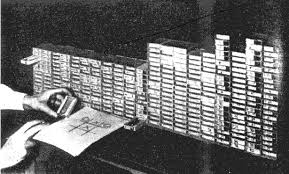
\includegraphics[scale=0.3]{14_rl/02_img/menace}
		};

		\node (C) at (2,0) {
			\begin{tikzpicture}[scale=0.15]
				\shade [ball color=black] (0,0) circle [radius=2cm];
			\end{tikzpicture}
		};

		\node (D) at (2,4) {
			\begin{tikzpicture}[scale=0.15]
				\draw[thick] (-6,2) -- (6,2);
				\draw[thick] (-6,-2) -- (6,-2);
				\draw[thick] (-2,-6) -- (-2,6);
				\draw[thick] (2,-6) -- (2,6);
				\draw[very thick] (-6,-6) -- (-6,6) -- (6,6) -- (6,-6) -- cycle;

				\node at (0,-4) {\textcolor{blue}{$\bm{\times}$}};
				\node at (0,0) {\textcolor{blue}{$\bm{\times}$}};
				\node at (0,4) {\textcolor{blue}{$\bm{\times}$}};
				\node at (-4,4) {\textcolor{red}{$\bm{\bigcirc}$}};
				\node at (4,4) {\textcolor{red}{$\bm{\bigcirc}$}};

				\shade [ball color=green] (-4,0) circle [radius=0.75cm];
				\shade [ball color=yellow] (-4,-4) circle [radius=0.75cm];
				\shade [ball color=blue] (4,-4) circle [radius=0.75cm];
				\shade [ball color=orange] (4,0) circle [radius=0.75cm];
			\end{tikzpicture}
		};

		\draw[->,thick] (A) -- node[left,align=left] {\footnotesize Choose matchbox \\ \footnotesize according to position} (B);
		\draw[->,thick] (B) -- node[above,align=left] {\footnotesize Pick a marble \\ \footnotesize from the matchbox} (C);
		\draw[->,thick] (C) -- node[right,align=left] {\footnotesize Execute move \\ \footnotesize according to 
			\\ \footnotesize marble} (D);
	
	\end{tikzpicture}
\end{figure}
\end{frame}


% Reinforcement Learning in MENACE
\begin{frame}{Reinforcement Learning in MENACE}{}
	\begin{itemize}
		\item \textbf{Initialization:} All moves are equally likely $\Rightarrow$ Each matchbox contains the same amount
			of marbles of each color
		\item \textbf{Learning algorithm}
		\begin{itemize}
			\item Game \Highlight{lost}: Marble is removed (negative reinforcement)
			\item Game \textcolor{green!80!black}{\textbf{won}}: Marble of corresponding color is added (positive reinforcement)
			\item \highlight{Remis}: Marbles are put back into the matchbox (no change)
		\end{itemize}
	\end{itemize}
	
	\vspace*{2mm}
	\begin{boxBlueNoFrame}
		$\bm{\Uparrow}$ Probability of successful moves is \highlight{increased} \\
		$\bm{\Downarrow}$ Probability of bad moves is \highlight{decreased}
	\end{boxBlueNoFrame}
\end{frame}


% Subsection: Reinforcement Learning Formalization
% --------------------------------------------------------------------------------------------------------
\subsection{Reinforcement Learning Formalization}

% Reinforcement Learning: Formalization
\begin{frame}{Reinforcement Learning: Formalization}{}
	\begin{itemize}
		\item Definitions
		\begin{itemize}
			\item $s \in \mathcal{S}$: state space (discrete or continuous)
			\item $a \in \mathcal{A}$: action space (discrete or continuous)
			\item $s_0 \in \mathcal{S}_0 \subseteq \mathcal{S}$: initial states
			\item $\delta : \mathcal{S} \times \mathcal{A} \rightarrow \mathcal{S}$: state transition function
				(deterministic or stochastic)
			\item $r : \mathcal{S} \times \mathcal{A} \rightarrow \mathbb{R}$: reward function
		\end{itemize}
		\item \highlight{Markov property} / \highlight{Markov Decision Process (MDP)}
		\begin{itemize}
			\item Rewards and state transitions depend on previous state only...
			\item ...and not how you got into this state (earlier states and actions don't matter)
		\end{itemize}
	\end{itemize}
\end{frame}


% Reinforcement Learning: Formalization (Ctd.)
\begin{frame}{Reinforcement Learning: Formalization (Ctd.)}{}
	\begin{itemize}
		\item The agent repeatedly chooses an action according to a \highlight{policy $\pi$}
		\begin{equation}
			\pi(s) = a
		\end{equation}
		\item This leads the agent into a new state $s'$
		\begin{equation}
			s' = \delta(s, \pi(s))
		\end{equation}
		\item The agent receives feedback (reinforcement) in some states
		\begin{itemize}
			\item Not necessarily in all states
			\item E.\,g. in a game there is usually no reward until the end (game is won or lost)
		\end{itemize}
	\end{itemize}
\end{frame}


% Reinforcement Learning: Formalization (Ctd.)
\begin{frame}{Reinforcement Learning: Formalization (Ctd.)}{}
	\begin{figure}
	\centering
	\begin{tikzpicture}[
		scale=0.4,
		every node/.style={scale=0.9}
	]
	
		\draw[thick] (0,0) -- (20,0) -- (20,3) -- (0,3) -- cycle;
		\node at (10,1.5) {\textbf{Environment}};

		\draw[thick] (5,6) -- (15,6) -- (15,12) -- (5,12) -- cycle;
		\node[align=center] at (10,9) {\textbf{Agent} \\ \footnotesize(has policy $\pi$)\normalsize};

		\draw[shorten >=0.2cm,shorten <=0.2cm,->,thick] (5,3) -- node[left] {State} (6,6);
		\draw[shorten >=0.2cm,shorten <=0.2cm,->,thick] (6,3) -- node[right] {Reward} (7,6);
		\draw[shorten >=0.2cm,shorten <=0.2cm,->,thick] (14,6) -- node[right] {Action} (15,3);

		\node (s0) at (4,-2) {$\bm{s_0}$};
		\node (s1) at (8,-2) {$\bm{s_1}$};
		\node (s2) at (12,-2) {$\bm{s_2}$};
		\node (s3) at (16,-2) {$\dots$};

		\draw[->] (s0) node[above right] {$a_0$} -- node[below right] {$r_0$} (s1);
		\draw[->] (s1) node[above right] {$a_1$} -- node[below right] {$r_1$} (s2);
		\draw[->] (s2) node[above right] {$a_2$} -- node[below right] {$r_2$} (s3);
	
	\end{tikzpicture}
\end{figure}
\end{frame}


% MENACE Formalization
\begin{frame}{MENACE Formalization}{}
	\begin{tabbing}
		\hspace*{4cm}\= \kill
		\highlight{States} 				\> Matchboxes (discrete) \\[1mm]
		\highlight{Actions} 				\> Possible moves (discrete) \\[1mm]
		\highlight{Policy }				\> Prefer actions with higher number of marbles (stochastic) \\[1mm]
		\highlight{Reward} 				\> Game won / game lost \\[1mm]
		\highlight{Transition function}		\> Choose next matchbox according to rules (deterministic)
	\end{tabbing}
		
	\begin{boxBlueNoFrame}
		\textbf{Task:} Find a policy $\pi$ that maximizes the sum of future rewards ($\widehat{=}\ \pi^*$).
	\end{boxBlueNoFrame}
\end{frame}


% Learning Task
\begin{frame}{Learning Task}{}
	\begin{itemize}
		\item \textbf{Goal:} Maximize the \highlight{cumulative reward} for the \highlight{trajectory $\tau$}
			which a policy $\pi$ generates
		\begin{itemize}
			\item \textbf{Deterministic:} $\tau$ is always the same
			\item \textbf{Stochastic:} $\tau$ can differ (random elements included)
		\end{itemize}
		\item Cumulative reward:
		\begin{equation}
			R(\pi) = R(\tau^{\pi}) = \sum_{t=0}^{\infty} \gamma^t r(s_t, a_t)
		\end{equation}
		\item \highlight{Discount factor $\gamma$}: Immediate rewards are weighted higher,
			rewards further in the future are discounted (exponentially)
	\end{itemize}
\end{frame}


% Learning Task (Ctd.)
\begin{frame}{Learning Task (Ctd.)}{}
	\begin{itemize}
		\item Rewards $t$ time steps in the future are discounted exponentially by a factor of $\gamma^t$
		\item Value of $\gamma$:
		\begin{itemize}
			\item $0 \le \gamma \le 1$
			\item $\gamma = 0$: Only immediate rewards are taken into account
			\item $\gamma = 1$: Future rewards are given same emphasis as immediate rewards
		\end{itemize}
		\item Usually, $\gamma$ is set to a value close to 1 (0.99, 0.98, 0.95, ...)
		\item Immediate rewards are usually preferred
	\end{itemize}
\end{frame}


% How to compute $R(\tau^{\pi})$?
\begin{frame}{How to compute $R(\tau^{\pi})$?}{}
	\vspace*{-8mm}
	\begin{align*}
		R(\tau^{\pi}) 	&= \sum_{t=0}^{\infty} \gamma^t r(s_t, a_t) \\
					&= r(s_0, a_0) + \gamma r(s_1, a_1) + \gamma^2 r(s_2, a_2) + \dots \\
					&= r(s_0, \pi(s_0)) + \sum_{t=1}^{\infty} \gamma^t r(\delta(s_{t-1}, \pi(s_{t-1})), \pi(s_t)) \\
					&= V^{\pi}(s_0)
	\end{align*}

	\vspace*{-2mm}
	\begin{itemize}
		\item $V$ is called the `value' of the first state
		\item \highlight{Value function}: Reward when starting in state $s_0$ and following policy $\pi$
	\end{itemize}
\end{frame}


% Optimal Policies and Value Functions
\begin{frame}{Optimal Policies and Value Functions}{}
	\begin{itemize}
		\item The optimal policy is denoted by $\pi^*$
		\item The optimal policy has the highest expected value for all states:
		\begin{align*}
			\pi^*(s) 	&= \argmax_{\pi} V^{\pi}(s) \quad \forall s \\
					&= \argmax_{a \in \mathcal{A}} r(s, a) + \gamma V^{\pi^*}(\delta(s, a)) \quad \forall s
		\end{align*}
		\item Always select the action that maximizes the value function for the next step,
			when following $\pi^*$ afterwards
		\item \textbf{Problem:} \textbf{Recursive definition of $\pi^*$} requires \highlight{perfect knowledge}
	\end{itemize}
\end{frame}


% An illustrative Example [given perfect Knowledge]
\begin{frame}{An illustrative Example (given perfect Knowledge)}{}
	\divideTwo{0.60}{
		\begin{itemize}
			\item Each square represents a state
			\item Each arrow represents a possible action
			\item Small numbers refer to the reward $r(s, a)$ obtained by taking the action
			\item In this case: Reward is always set to 0, except when entering the goal state $\bm{\mathcal{G}}$
			\item $\bm{\mathcal{G}}$ is an absorbing state (impossible to get out again)
			\item $\gamma = 0.9$
		\end{itemize}
	}{0.39}{
		\vspace*{2mm}
		\begin{figure}
	\centering
	\begin{tikzpicture}[scale=0.75]
	
		\draw[very thick] (0,0) -- (6,0) -- (6,4) -- (0,4) -- cycle;
		\draw[thick] (2,0) -- (2,4); \draw (4,0) -- (4,4);
		\draw[thick] (0,2) -- (6,2);

		\draw[->,thick] (1.6,3.75) -- (2.4,3.75) node[right] {\tiny 0};
		\draw[->,thick] (2.4,3.45) -- (1.6,3.45) node[left] {\tiny 0};

		\draw[->,thick] (1.6,0.55) -- (2.4,0.55) node[right] {\tiny 0} ;
		\draw[->,thick] (2.4,0.25) -- (1.6,0.25) node[left] {\tiny 0} ;

		\draw[->,thick] (3.6,0.55) -- (4.4,0.55) node[right] {\tiny 0} ;
		\draw[->,thick] (4.4,0.25) -- (3.6,0.25) node[left] {\tiny 0};

		\draw[->,thick] (0.25,1.6) -- (0.25,2.4) node[above] {\tiny 0};
		\draw[->,thick] (0.55,2.4) -- (0.55,1.6) node[below] {\tiny 0};

		\draw[->,thick] (2.25,1.6) -- (2.25,2.4) node[above] {\tiny 0};
		\draw[->,thick] (2.55,2.4) -- (2.55,1.6) node[below] {\tiny 0};

		\draw[->,thick] (3.6,3.75) -- (4.4,3.75) node[right] {\tiny 100};
		\draw[->,thick] (4.25,1.6) -- (4.25,2.4) node[above] {\tiny 100};

		\node (G) at (5,3) {$\bm{\mathcal{G}}$};
		\draw[thick,->,shorten >=1pt] (G) to [out=270,in=360,loop,looseness=4.8] (G);
		\node at (5.4,2.6) {\tiny 0};

		\node at (1, 1) {$\bm{s_0}$};
		\node at (3, 1) {$\bm{s_1}$};
		\node at (5, 1) {$\bm{s_2}$};

		\node at (1, 3) {$\bm{s_3}$};
		\node at (3, 3) {$\bm{s_4}$};
	
	\end{tikzpicture}
\end{figure}
	}
\end{frame}


% An illustrative Example (given perfect Knowledge) (Ctd.)
\begin{frame}{An illustrative Example [given perfect Knowledge] (Ctd.)}{}
	In this case we can derive the optimal policy $\pi^*$ directly,
		e.\,g. $s_0 \rightarrow s_3 \rightarrow s_4 \rightarrow \mathcal{G}$
	\divideTwo{0.60}{
		\begin{alignat*}{2}
			V^{\pi^*}(s_0) &= 0 + \gamma 0 + \gamma^2 100 + \gamma^3 0 + \dots 	&&= \bm{81}
			\\[2mm]
			V^{\pi^*}(s_1) &= 0 + \gamma 100 + \gamma^2 0 + \gamma^3 0 + \dots 	&&= \bm{90}
			\\[2mm]
			V^{\pi^*}(s_2) &= 100 + \gamma 0 + \gamma^2 0 + \gamma^3 0 + \dots	&&= \bm{100}
			\\[2mm]
			V^{\pi^*}(s_3) &= 0 + \gamma 100 + \gamma^2 0 + \gamma^3 0 + \dots 	&&= \bm{90}
			\\[2mm]
			V^{\pi^*}(s_4) &= 100 + \gamma 0 + \gamma^2 0 + \gamma^3 0 + \dots	&&= \bm{100}
		\end{alignat*}
	}{0.39}{
		\vspace*{2mm}
		\begin{figure}
	\centering
	\begin{tikzpicture}[scale=0.75]
	
		\draw[very thick] (0,0) -- (6,0) -- (6,4) -- (0,4) -- cycle;
		\draw[thick] (2,0) -- (2,4); \draw (4,0) -- (4,4);
		\draw[thick] (0,2) -- (6,2);

		\draw[->,thick] (1.6,3.75) -- (2.4,3.75);
		\draw[->,thick] (2.4,3.45) -- (1.6,3.45);

		\draw[->,thick] (1.6,0.55) -- (2.4,0.55);
		\draw[->,thick] (2.4,0.25) -- (1.6,0.25);

		\draw[->,thick] (3.6,0.55) -- (4.4,0.55);
		\draw[->,thick] (4.4,0.25) -- (3.6,0.25);

		\draw[->,thick] (0.25,1.6) -- (0.25,2.4);
		\draw[->,thick] (0.55,2.4) -- (0.55,1.6);

		\draw[->,thick] (2.25,1.6) -- (2.25,2.4);
		\draw[->,thick] (2.55,2.4) -- (2.55,1.6);

		\draw[->,thick] (3.6,3.75) -- (4.4,3.75);
		\draw[->,thick] (4.25,1.6) -- (4.25,2.4);

		\node (G) at (5,3) {$\bm{\mathcal{G}}$};
		\draw[thick,->,shorten >=1pt] (G) to [out=270,in=360,loop,looseness=4.8] (G);
		\node at (4.3,3) {\textbf{0}};

		\node at (1, 1) {\textbf{81}};
		\node at (3, 1) {\textbf{90}};
		\node at (5, 1) {\textbf{100}};

		\node at (1, 3) {\textbf{90}};
		\node at (3, 3) {\textbf{100}};
	
	\end{tikzpicture}
\end{figure}
	}
\end{frame}


% Section: Basic Algorithms
%______________________________________________________________________
\section{Basic Algorithms}
\makedivider{Basic Algorithms}

% Subsection: How to learn the optimal Policy?
% --------------------------------------------------------------------------------------------------------
\subsection{How to learn the optimal Policy?}

% How to learn the optimal Policy?
\begin{frame}{How to learn the optimal Policy?}{}
	\begin{itemize}
		\item W/o perfect knowledge it's difficult to learn the optimal policy directly, since training data of the
			form $\langle s, a \rangle$ is not available (\textbf{$\ne$ supervised learning})
		\item The only information at the agent's disposal is the sequence of observed immediate rewards: 
		\begin{equation*}
			r_0 \longrightarrow r_1 \longrightarrow r_2 \longrightarrow r_3 \longrightarrow r_4 \longrightarrow \dots
		\end{equation*}
		\item What evaluation function should be learned?
		\begin{itemize}
			\item One obvious choice is $V^{\pi^*}$
			\item The agent should prefer state $s_1$ over $s_2$, if $V^{\pi^*}(s_1) > V^{\pi^*}(s_2)$
		\end{itemize}
	\end{itemize}
\end{frame}


% How to learn the optimal Policy? (Ctd.)
\begin{frame}{How to learn the optimal Policy? (Ctd.)}{}
	\begin{itemize}
		\item The optimal action in state $s$ is action $a$ that maximizes the sum of the immediate reward $r(s, a)$,
			plus the value of $V^{\pi^*}$ of the immediate successor, discounted by $\gamma$:
		\begin{equation}
			\pi^*(s) = \argmax_{a \in \mathcal{A}} r(s, a) + \gamma V^{\pi^*}(\delta(s, a))
		\end{equation}
		\item \textbf{Problem:}
		\begin{itemize}
			\item In order to calculate $V^{\pi^*}$ the agent needs to know $\delta(s, a)$ and $r(s, a)$
			\item Learning $V^{\pi*}$ is of no use, since the equation cannot be evaluated
		\end{itemize}
		\item $\overset{Remedy}{\Longrightarrow}$ Value iteration, policy iteration, Q-Learning, SARSA, ...
	\end{itemize}
\end{frame}


% Subsection: Value Iteration
% --------------------------------------------------------------------------------------------------------
\subsection{Value Iteration}

% Value Iteration Algorithm
\begin{frame}{Value Iteration Algorithm}{}
	\begin{algorithm}[H]
		\footnotesize
		\DontPrintSemicolon
		\KwIn{environment $\mathcal{E} = (\mathcal{S}, \mathcal{A})$}
		\KwOut{optimal policy $\pi$}
		\vspace*{1mm}
 		Initialize $V(s) \in \mathbb{R}$ arbitrarily for all $s \in \mathcal{S}$\;
 		\While{$\Delta > \varepsilon$}{
 			$\Delta \longleftarrow 0$\;
 			\ForEach{$s \in \mathcal{S}$}{
 				$v \longleftarrow V(s)$\;
				$V(s) \longleftarrow \max_a \sum_{s', r} p(s', r \vert s, a)[r + \gamma V(s')]$\;
				$\Delta \longleftarrow \max(\Delta, \vert v - V(s) \vert)$\;
 			}
 		}
		\textbf{return} $\pi$ such that $\pi(s) = \argmax_a \sum_{s', r} p(s', r \vert s, a)[r + \gamma V(s')]$\;
 		\caption{Value Iteration}
	\end{algorithm}
\end{frame}


% Backup Diagram for Value Iteration
\begin{frame}{Backup Diagram for Value Iteration}{}
	\begin{figure}
		\centering
		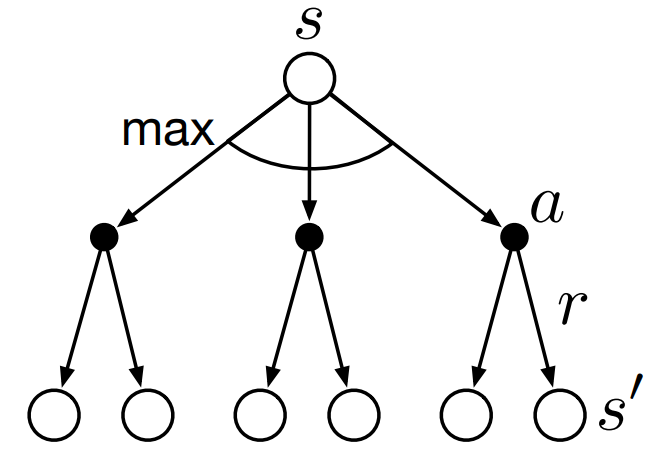
\includegraphics[scale=0.45]{14_rl/02_img/backup_diagram_value_iteration}
	\end{figure}
\end{frame}


% Subsection: Policy Iteration
% --------------------------------------------------------------------------------------------------------
\subsection{Policy Iteration}

% Policy Iteration
\begin{frame}{Policy Iteration}{}
	\begin{itemize}
		\item Initialize a policy randomly, find its value function and iterate
		\begin{itemize}
			\item \highlight{Policy evaluation}: Find the value function of the current policy
			\item \highlight{Policy improvement}: Find a better policy based on the current one
		\end{itemize}
		\item Select the action that maximizes the value function of the current policy:
		\begin{equation}
			\pi'(s) = \argmax_{a \in \mathcal{A}} r(s, a) + \gamma V^{\pi}(\delta(s, a))
		\end{equation}
		\item This leads to a sequence of improving policies:
		\begin{equation*}
			\pi^0(s) \longrightarrow V^{\pi^0}(s) \longrightarrow \pi^1(s) \longrightarrow V^{\pi^1}(s)
			\longrightarrow \dots \longrightarrow \pi^*(s)
		\end{equation*}
	\end{itemize}
\end{frame}


% Policy Iteration (Ctd.)
\begin{frame}{Policy Iteration (Ctd.)}{}
	\begin{figure}
		\centering
		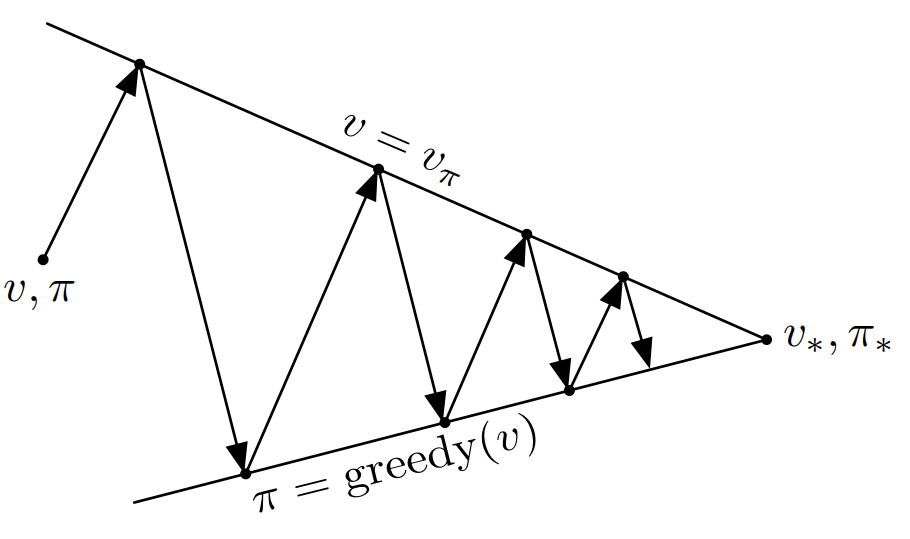
\includegraphics[scale=0.4]{14_rl/02_img/policy_iteration}
	\end{figure}
\end{frame}


% Policy Improvement Theorem
\begin{frame}{Policy Improvement Theorem}{}
	\begin{boxBlue}
		\highlight{Policy improvement theorem:} \\[2mm]
		\footnotesize
		\highlight{If it is true that selecting the first action in each state according to a policy $\pi'$ and continuing
		with policy $\pi$ is better than always following $\pi$, then $\pi'$ is a better policy than $\pi$.}
	\end{boxBlue}
\end{frame}


% Policy Iteration Algorithm
\begin{frame}{Policy Iteration Algorithm}{}
	\begin{algorithm}[H]
		\footnotesize
		\DontPrintSemicolon
		\KwIn{environment $\mathcal{E} = (\mathcal{S}, \mathcal{A})$}
		\KwOut{optimal policy $\pi$}
		\vspace*{1mm}
 		Initialize $V(s) \in \mathbb{R}$ and $\pi(s) \in \mathcal{A}$ arbitrarily for all $s \in \mathcal{S}$\;

		$policy\_stable \longleftarrow false$\;
		\While{$not\ policy\_stable$}{
			$V_{new} \longleftarrow PolicyEvaluation(\pi, V, \varepsilon=0.001)$\;
			$\pi, policy\_stable \longleftarrow PolicyImprovement(V_{new})$\;
			$V \longleftarrow V_{new}$
		}

		\textbf{return} $\pi$\;
 		\caption{Policy Iteration (deterministic case)}
	\end{algorithm}
\end{frame}


% Policy Evaluation and Policy Improvement
\begin{frame}{Policy Evaluation and Policy Improvement}{}
	\begin{algorithm}[H]
		\footnotesize
		\DontPrintSemicolon
		\KwIn{current policy $\pi$, current value function $V$, threshold $\varepsilon$}
		\KwOut{updated value function $V$}
		\vspace*{1mm}
		\While{$\Delta > \varepsilon$}{
 				$\Delta \longleftarrow 0$\;
 				\ForEach{$s \in \mathcal{S}$}{
 					$v \longleftarrow V(s)$\;
				$V(s) \longleftarrow \sum_{s', r} p(s', r \vert s, \pi(s))[r + \gamma V^{\pi}(s')]$\;
				$\Delta \longleftarrow \max(\Delta, \vert v - V(s) \vert)$\;
 				}
 			}
		\textbf{return} $V$
 			\caption{Policy Evaluation}
	\end{algorithm}
\end{frame}


% Policy Evaluation and Policy Improvement
\begin{frame}{Policy Evaluation and Policy Improvement}{}
	\begin{algorithm}[H]
		\footnotesize
		\DontPrintSemicolon
		\KwIn{updated value function $V$}
		\KwOut{updated policy $\pi$, boolean flag $policy\_stable$}
		\vspace*{1mm}
		$policy\_stable \longleftarrow true$\;
		\ForEach{$s \in \mathcal{S}$}{
			$old\_action \longleftarrow \pi(s)$\;
			$\pi(s) \longleftarrow \argmax_{a}\sum_{s', r} p(s', r \vert s, a)[r + \gamma V^{\pi}(s')]$\;
			\If{$old\_action \ne \pi(s)$}{
				$policy\_stable \longleftarrow false$\;
			}
		}
		\textbf{return} $\pi, policy\_stable$
 			\caption{Policy Improvement}
	\end{algorithm}
\end{frame}


% Backup Diagram for Policy Iteration
\begin{frame}{Backup Diagram for Policy Iteration}{}
	\begin{figure}
		\centering
		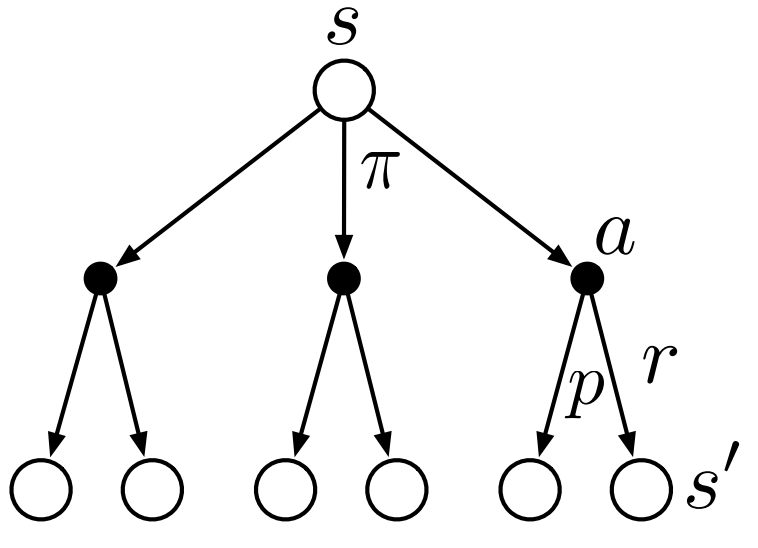
\includegraphics[scale=0.375]{14_rl/02_img/backup_diagram_policy_iteration}
	\end{figure}
\end{frame}


% Policy Iteration Example: Grid World I
\begin{frame}[plain]{Policy Iteration Example: Grid World I}{}
	\begin{figure}
		\centering
		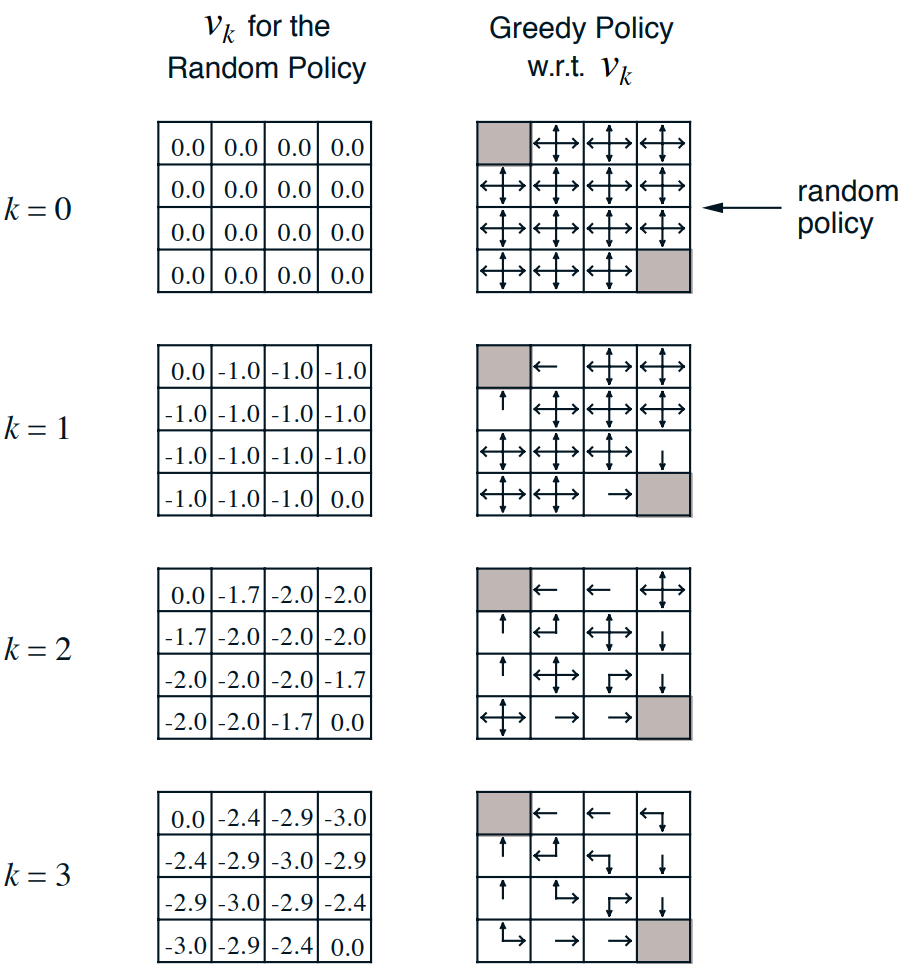
\includegraphics[scale=0.275]{14_rl/02_img/policy_iteration_gridworld}
	\end{figure}
\end{frame}


% Policy Iteration Example: Grid World II
\begin{frame}[plain]{Policy Iteration Example: Grid World II}{}
	\begin{figure}
		\centering
		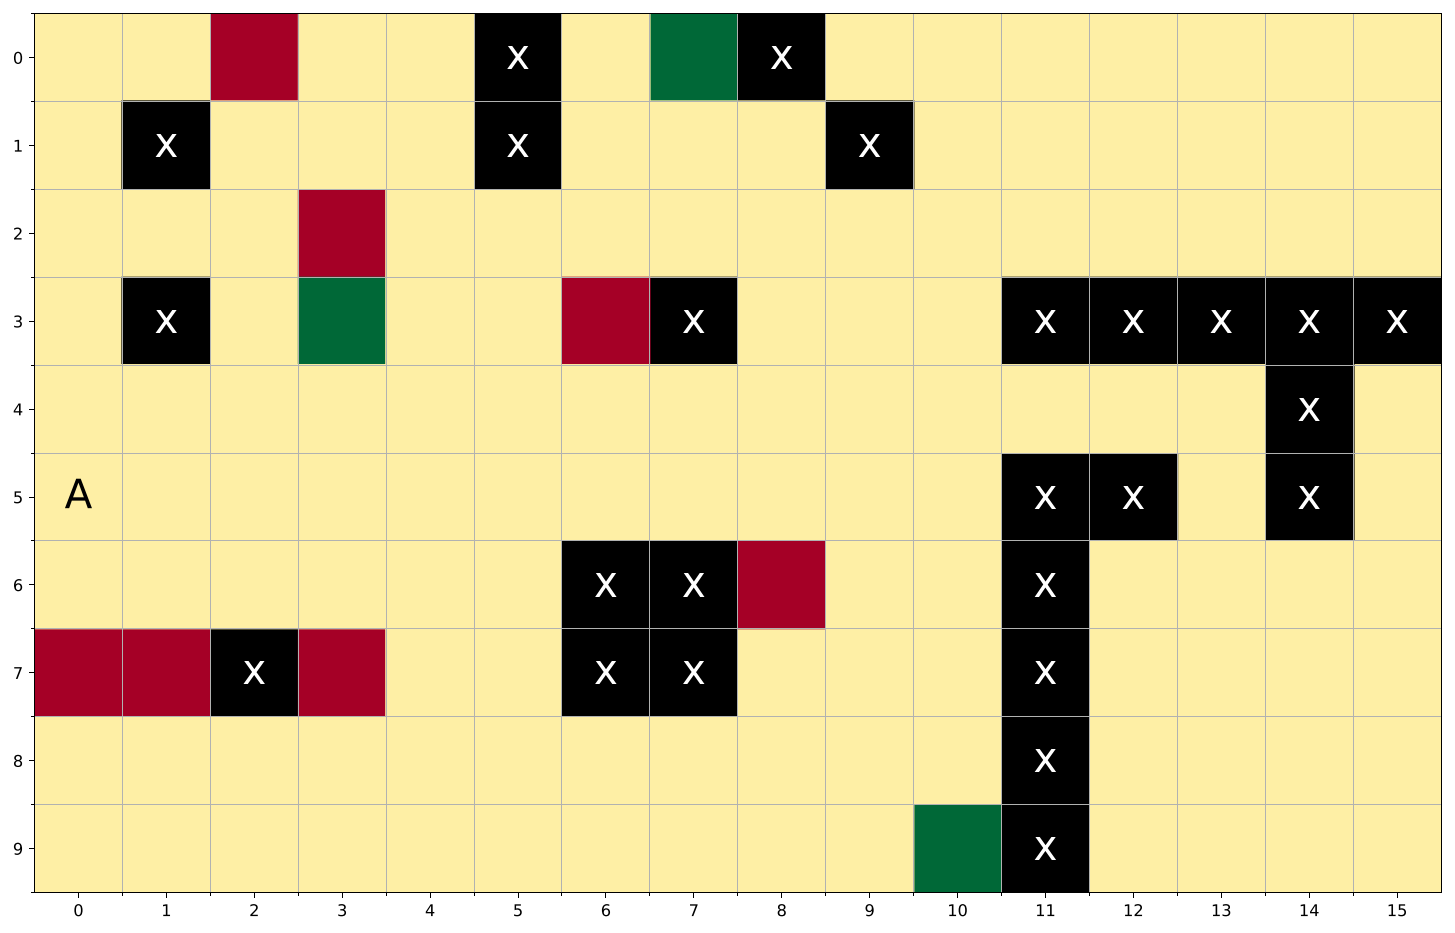
\includegraphics[scale=0.3]{14_rl/02_img/grid_world}
	\end{figure}
\end{frame}


% Policy Iteration Example: Grid World II
\begin{frame}[plain]{Policy Iteration Example: Grid World II (solved)}{}
	\begin{figure}
		\centering
		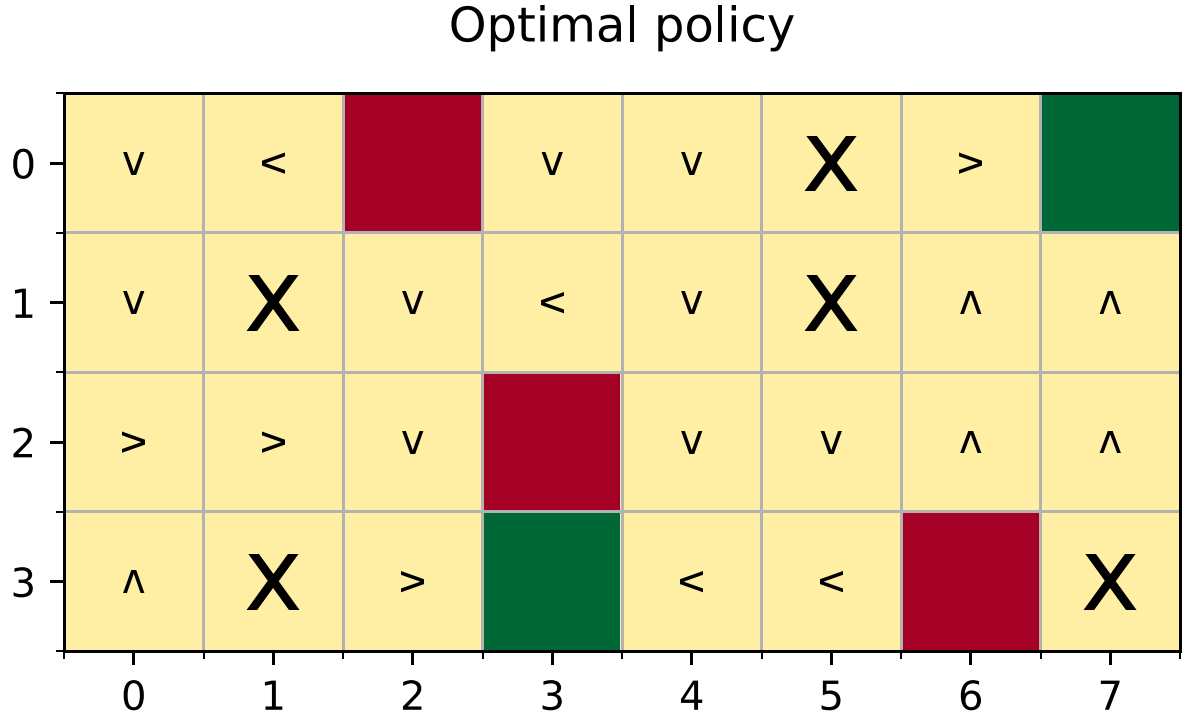
\includegraphics[scale=0.3]{14_rl/02_img/optimal_policy_pi}
	\end{figure}
\end{frame}


% Subsection: $Q$-Learning
% --------------------------------------------------------------------------------------------------------
\subsection{$Q$-Learning}

% Q-Learning
\begin{frame}{$Q$-Learning}{}
	\begin{itemize}
		\item $Q(s, a) \equiv$ maximum discounted cumulative reward that can be achieved starting from state $s$
			and applying action $a$ as the first action:
		\begin{equation}
			Q(s, a) = r(s, a) + \gamma V^{\pi^*}(\delta(s, a)) \qquad \text{\textit{looks familiar?}}
		\end{equation}
		\item Formula for $\pi^*$ can be rewritten in terms of $Q(s, a)$:
		\begin{equation}
			\pi^*(s) = \argmax_{a \in \mathcal{A}} Q(s, a)
		\end{equation}
		\item \highlight{This rewrite is important:} Learning the $Q$-function the agent can select optimal actions
			without any knowledge of $r$ and $\delta$
	\end{itemize}
\end{frame}


% Q-Learning (Ctd.)
\begin{frame}{$Q$-Learning (Ctd.)}{}
	\begin{itemize}
		\item By always choosing the action with the maximum $Q$-value...
		\begin{equation*}
			\argmax_{a \in \mathcal{A}} Q(s, a)
		\end{equation*}
		\item ...we maximize the expected cumulative reward
		\item What may seem surprising: Local optimal choices lead to a global optimal solution
	\end{itemize}

	\vspace*{2mm}
	\begin{boxBlueNoFrame}
		Learning the $Q$-function corresponds to learning the optimal policy $\pi^*$
	\end{boxBlueNoFrame}
\end{frame}


% Algorithm for $Q$-Learning
\begin{frame}{Algorithm for $Q$-Learning}{}
	\textbf{How can $Q$ be learned?}
	\begin{itemize}
		\item We learn the $Q$-function by iterative approximation
		\item Note the close relationship of $Q$ and $V^{\pi^*}$:
		\begin{equation}
			V^{\pi^*}(s) = \max_{a' \in \mathcal{A}} Q(s, a')
		\end{equation}
		\item Therefore, $Q(s, a)$ can be expressed in terms of itself: \highlight{Bellman equation}
	\end{itemize}
	
	\begin{boxBlueNoFrame}
		\begin{equation}
			Q(s, a) = r(s, a) + \gamma \max_{a' \in \mathcal{A}} Q(\delta(s, a), a')
		\end{equation}
	\end{boxBlueNoFrame}
\end{frame}


% Algorithm for $Q$-Learning (Ctd.)
\begin{frame}{Algorithm for $Q$-Learning (Ctd.)}{}
	\divideTwo{0.60}{
		\begin{itemize}
			\item $\widehat{Q}$ denotes the agent's current estimate of the true $Q$-value (which is unknown)
			\item The $Q$-function is represented by a table (one entry per state-action pair)
			\item Initially, the table is filled with random numbers or zeroes
			\item \Highlight{The table may become large, if there are many states and actions}
		\end{itemize}
	}{0.39}{
		\vspace*{2mm}
		\begin{table}[h]
	\scalebox{0.8}{
		\renewcommand{\arraystretch}{1.3}
		\begin{tabular}{| c | c |}
			\hline
			\textbf{State-action pair} &
			$\bm{\widehat{Q}}$-\textbf{value} \\
			\hline\hline
			$\langle s_0, a_0 \rangle$ & $\widehat{Q}(s_0, a_0)$ \\ \hline
			$\langle s_0, a_1 \rangle$ & $\widehat{Q}(s_0, a_1)$ \\ \hline
			$\langle s_1, a_0 \rangle$ & $\widehat{Q}(s_1, a_0)$ \\ \hline
			$\langle s_1, a_1 \rangle$ & $\widehat{Q}(s_1, a_1)$ \\ \hline
			$\dots$ 					& $\dots$			  \\ \hline
		\end{tabular}
	}
\end{table}














	}	
\end{frame}


% Algorithm for $Q$-Learning (Ctd.)
\begin{frame}{Algorithm for $Q$-Learning (Ctd.)}{}
	\begin{itemize}
		\item The agent repeatedly observes the current state $s$, chooses some action $a$, executes it and
			observes $r$ as well as the new state $s'$
		\item Update the table entry for $\widehat{Q}(s, a)$ according to the Bellman equation
		\item The agent doesn't have to know $\delta(s, a)$ and $r(s, a)$
		\item Instead, it executes some actions and observes what happens
		\item In the limit, $\widehat{Q}$ will converge towards the actual $Q$-function \textbf{iff}...
		\begin{itemize}
			\item ...the system can be modeled as a deterministic MDP...
			\item ...\textbf{and} the reward function is bounded...
			\item ...\textbf{and} each state-action pair is visited infinitely often
		\end{itemize}
	\end{itemize}
\end{frame}


% Algorithm for $Q$-Learning (Ctd.)
\begin{frame}{Algorithm for $Q$-Learning (Ctd.)}{}
	\begin{algorithm}[H]
		\footnotesize
		\DontPrintSemicolon
 		\ForEach(\tcp*[h]{initialize table entries with zeroes}){$\langle s, a \rangle$}{
 			$\widehat{Q}(s, a) \longleftarrow 0$ \tcp*[h]{Alternative: Initialize with random numbers}\;
 		}
		\While(\tcp*[h]{endless loop}){true}{
  			Observe current state $s$\;
  			Select an action $a$ and execute it\;
  			Receive the immediate reward $r$\;
  			Observe the new state $s'$\;
  			Update the table entry for $\widehat{Q}(s, a)$:
  				$\widehat{Q}(s, a) \longleftarrow r + \gamma \max_{a' \in \mathcal{A}} \widehat{Q}(s', a')$\;
  			$s \longleftarrow s'$\;
 		}
 		\caption{Learning the $Q$-function}
	\end{algorithm}
\end{frame}


% $Q$-Learning: An illustrative Example
\begin{frame}{$Q$-Learning: An illustrative Example}{}
	\begin{figure}
	\centering
	\begin{tikzpicture}[scale=0.6]
	
		\node (A) at (-5,0) {
			\begin{tikzpicture}[scale=0.75]
				\draw[very thick] (0,0) -- (6,0) -- (6,4) -- (0,4) -- cycle;
				\draw[thick] (2,0) -- (2,4); \draw (4,0) -- (4,4);
				\draw[thick] (0,2) -- (6,2);
			
				\draw[->,thick] (1.6,3.75) -- (2.4,3.75) node[right] {\tiny 73};
				\draw[->,thick] (2.4,3.45) -- (1.6,3.45) node[left] {\tiny 66};
	
				\draw[->,thick] (3.6,3.75) -- (4.4,3.75) node[right] {\tiny 100};

				\draw[->,thick] (2.55,2.4) -- (2.55,1.6) node[below] {\tiny 81};

				\node at (1, 2.75) {\huge{$\bm{\smiley}$}};
			\end{tikzpicture}
		};

		\node (B) at (5,0) {
			\begin{tikzpicture}[scale=0.75]
				\draw[very thick] (0,0) -- (6,0) -- (6,4) -- (0,4) -- cycle;
				\draw[thick] (2,0) -- (2,4); \draw (4,0) -- (4,4);
				\draw[thick] (0,2) -- (6,2);
			
				\draw[->,thick] (1.6,3.75) -- (2.4,3.75) node[right] {\tiny \highlight{90}};
				\draw[->,thick] (2.4,3.45) -- (1.6,3.45) node[left] {\tiny 66};
	
				\draw[->,thick] (3.6,3.75) -- (4.4,3.75) node[right] {\tiny 100};

				\draw[->,thick] (2.55,2.4) -- (2.55,1.6) node[below] {\tiny 81};

				\node at (3, 2.75) {\huge{$\bm{\smiley}$}};
			\end{tikzpicture}
		};

		\draw[->] (A) -- node[above] {$\bm{a_{right}}$} (B);
	
	\end{tikzpicture}
\end{figure}
	\vspace*{-2mm}
	\begin{align*}
		\widehat{Q}(s_3, a_{right}) 	&\longleftarrow r + \gamma \max_{a' \in \mathcal{A}} \widehat{Q}(s_4, a') \\
								&\longleftarrow 0 + 0.9 \max_{a' \in \mathcal{A}}\{66,81,100\} \\
								&\longleftarrow 90
	\end{align*}
\end{frame}


% $Q$-Learning: An illustrative Example (Ctd.)
\begin{frame}{$Q$-Learning: An illustrative Example (Ctd.)}{}
	\begin{itemize}
		\item Each time the agent makes a move, the $Q$-value estimates are \textbf{propagated backwards}
			from the new state $s'$ to the old state $s$
		\item The immediate reward is used to \textbf{augment} the propagated values of $\widehat{Q}$
		\item Since there is an absorbing goal state $\bm{\mathcal{G}}$, there will be a series of episodes
		\item \textbf{One episode:}
		\begin{enumerate}
			\item Initialize the agent at a random state
			\item The episode ends as soon as the goal state $\bm{\mathcal{G}}$ is reached
			\item Repeat until convergence (\texttt{goto 1})
		\end{enumerate}
	\end{itemize}
\end{frame}


% $Q$-Learning: An illustrative Example (Ctd.)
\begin{frame}{$Q$-Learning: An illustrative Example (Ctd.)}{}
	\begin{figure}
	\centering
	\begin{tikzpicture}[scale=1.2]
	
		\draw[very thick] (0,0) -- (6,0) -- (6,4) -- (0,4) -- cycle;
		\draw[thick] (2,0) -- (2,4); \draw (4,0) -- (4,4);
		\draw[thick] (0,2) -- (6,2);

		\draw[->,thick,myblue1] (1.6,3.75) -- (2.4,3.75) node[right] {\tiny 90};
		\draw[->,thick] (2.4,3.45) -- (1.6,3.45) node[left] {\tiny 81};

		\draw[->,thick,myblue1] (1.6,0.55) -- (2.4,0.55) node[right] {\tiny 81} ;
		\draw[->,thick] (2.4,0.25) -- (1.6,0.25) node[left] {\tiny 72} ;

		\draw[->,thick,myblue1] (3.6,0.55) -- (4.4,0.55) node[right] {\tiny 90} ;
		\draw[->,thick] (4.4,0.25) -- (3.6,0.25) node[left] {\tiny 81};

		\draw[->,thick,myblue1] (0.25,1.6) -- (0.25,2.4) node[above] {\tiny 81};
		\draw[->,thick] (0.55,2.4) -- (0.55,1.6) node[below] {\tiny 72};

		\draw[->,thick,myblue1] (2.25,1.6) -- (2.25,2.4) node[above] {\tiny 90};
		\draw[->,thick] (2.55,2.4) -- (2.55,1.6) node[below] {\tiny 81};

		\draw[->,thick,myblue1] (3.6,3.75) -- (4.4,3.75) node[right] {\tiny 100};
		\draw[->,thick,myblue1] (4.25,1.6) -- (4.25,2.4) node[above] {\tiny 100};

		\node (G) at (5,3) {$\bm{\mathcal{G}}$};
		\draw[thick,->,shorten >=1pt,myblue1] (G) to [out=270,in=360,loop,looseness=4.8] (G);
		\node[myblue1] at (5.2,2.6) {\tiny 0};

		\node at (1, 1) {$\bm{s_0}$};
		\node at (3, 1) {$\bm{s_1}$};
		\node at (5, 1) {$\bm{s_2}$};

		\node at (1, 3) {$\bm{s_3}$};
		\node at (3, 3) {$\bm{s_4}$};
	
	\end{tikzpicture}
\end{figure}
\end{frame}


% Subsection: SARSA: State-Action-Reward-State-Action
% --------------------------------------------------------------------------------------------------------
\subsection{SARSA: State-Action-Reward-State-Action}

% SARSA: State-Action-Reward-State-Action
\begin{frame}{SARSA: State-Action-Reward-State-Action}{}
	\begin{itemize}
		\item SARSA is very similar to $Q$-learning
		\item The abbreviation stands for `\highlight{S}tate-\highlight{A}ction-\highlight{R}eward-\highlight{S}tate-\highlight{A}ction'
		\item It refrains from calculating the `$\max$' in the formula
		\item Instead it uses the current policy (\highlight{on-policy update})
	\end{itemize}
	
	\vspace*{2mm}
	\begin{boxBlueNoFrame}
		\begin{equation}
			\widehat{Q}(s, a) \longleftarrow r(s, a) + \gamma \widehat{Q}(\underbracket{\delta(s, a)}_{=s'}, \pi(s'))
		\end{equation}
	\end{boxBlueNoFrame}
\end{frame}


% Backup Diagrams for $Q$-Learning and SARSA
\begin{frame}{Backup Diagrams for $Q$-Learning and SARSA}{}
	\begin{figure}
		\centering
		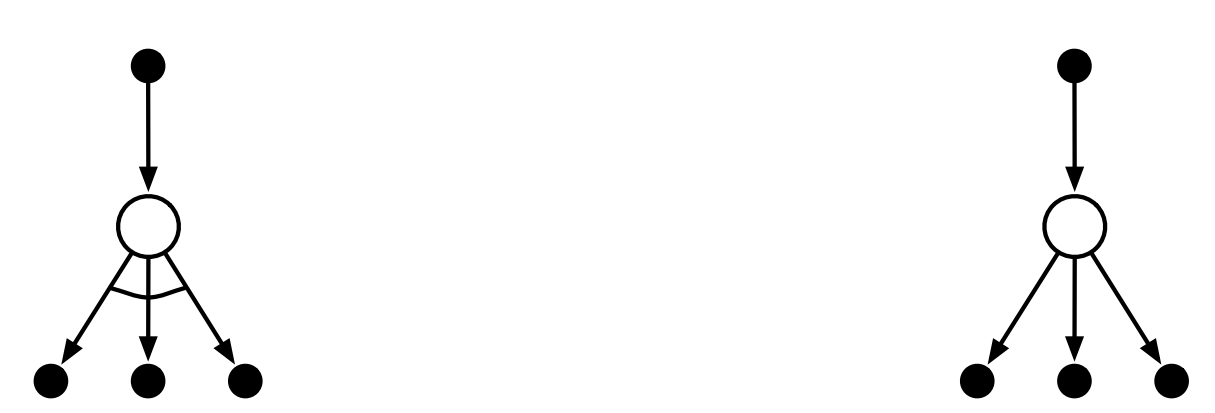
\includegraphics[scale=0.35]{14_rl/02_img/backup_diagram_q_learning_sarsa}
		\caption{Backup diagrams of $Q$-learning (left) and SARSA (right)}
	\end{figure}
\end{frame}


% Section: Miscellaneous
%______________________________________________________________________
\section{Miscellaneous}
\makedivider{Miscellaneous}

% Subsection: Exploitation vs. Exploration
% --------------------------------------------------------------------------------------------------------
\subsection{Exploitation vs. Exploration}

% Exploitation vs. Exploration
\begin{frame}{Exploitation vs. Exploration}{}
	\begin{itemize}
		\item By always picking the best action the agent runs the risk of overcommitting to actions that were found
			during early training
		\item \Highlight{It fails to explore other actions that might be even better}
	\end{itemize}

	\vspace*{2mm}
	\divideTwo{0.49}{
		\begin{itemize}
			\item \textbf{Exploitation:}
			\begin{itemize}
				\item Use the action the agent assumes to be the best one
				\item Approximate the optimal policy
			\end{itemize}
		\end{itemize}
	}{0.49}{
		\begin{itemize}
			\item \textbf{Exploration:}
			\begin{itemize}
				\item `Optimal action' may be wrong due to approximation errors
				\item Try a sub-optimal one
			\end{itemize}
		\end{itemize}
	}
	
	\vspace*{2mm}
	\begin{boxBlueNoFrame}
		\highlight{There is an exploitation $\bm{\Leftrightarrow}$ exploration trade-off!}
	\end{boxBlueNoFrame}
\end{frame}


% Exploitation vs. Exploration (Ctd.)
\begin{frame}{Exploitation vs. Exploration (Ctd.)}{}
	\begin{itemize}
		\item $\bm{\varepsilon}$\textbf{-greedy} (small $\varepsilon \Rightarrow$ exploitation)
		\begin{equation}
			p(a_i \vert s) =
			\begin{cases}
				1 - \varepsilon + \frac{\varepsilon}{\vert \mathcal{A} \vert} & 
					\text{\textbf{if}}\ a_i = \argmax_{a \in \mathcal{A}} \widehat{Q}(s, a) \\
				\frac{\varepsilon}{\vert \mathcal{A} \vert} &
					\text{\textbf{otherwise}}
			\end{cases}
		\end{equation}
		\item \textbf{Softmax} (actions with high $\widehat{Q}$-values get a higher probability)
		\begin{equation}
			p(a_i \vert s) = \frac{k^{\widehat{Q}(s, a_i)}}{\sum_j k^{\widehat{Q}(s, a_j)}}
			\qquad k > 0 \quad \text{(large $k \Rightarrow$ exploitation)}
		\end{equation}
	\end{itemize}
\end{frame}


% Subsection: Non-Deterministic Rewards and Actions
% --------------------------------------------------------------------------------------------------------
\subsection{Non-Deterministic Rewards and Actions}

% Non-Deterministic Rewards and Actions
\begin{frame}{Non-Deterministic Rewards and Actions}{}
	\begin{itemize}
		\item So far we have only considered the deterministic case
		\item \textbf{What if the environment is non-deterministic?}
		\begin{itemize}
			\item E.\,g. in Backgammon, each move involves a roll of the dice $\Rightarrow \delta(s, a)$ varies
			\item Also, the rewards may change $\Rightarrow r(s, a)$ varies
		\end{itemize}
	\end{itemize}

	\begin{figure}
		\centering
		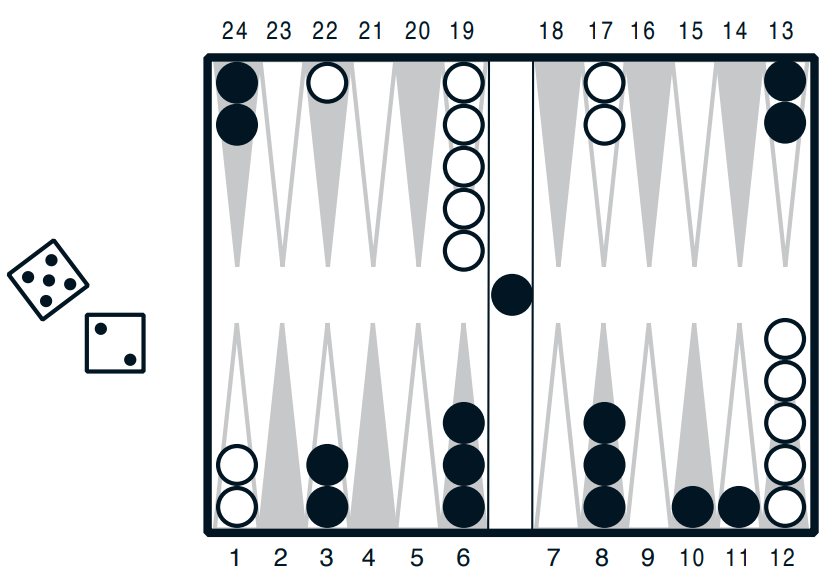
\includegraphics[scale=0.2]{14_rl/02_img/backgammon}
	\end{figure}
\end{frame}


% Non-Deterministic Rewards and Actions (Ctd.)
\begin{frame}{Non-Deterministic Rewards and Actions (Ctd.)}{}
	\begin{itemize}
		\item $\delta(s, a)$ and $r(s, a)$ can be viewed as first producing a probability distribution over the outcomes based
			on $s$ and $a$, and then drawing an outcome at random according to this distribution
		\item If these probability distributions depend solely on $s$ and $a$ (not on earlier states or actions), then
			the system is called \highlight{non-deterministic Markov decision process}
	\end{itemize}

	\vspace*{2mm}
	\begin{boxBlueNoFrame}
		The $Q$-learning algorithm has to be modified in order to be able to handle the non-deterministic case.
	\end{boxBlueNoFrame}
\end{frame}


% Non-Deterministic Rewards and Actions (Ctd.)
\begin{frame}{Non-Deterministic Rewards and Actions (Ctd.)}{}
	\begin{itemize}
		\item Restate the agent's objective $\Rightarrow$ Redefine the value $V^{\pi}$ of a policy $\pi$
			to be the expected value (solve e.\,g. by using \highlight{Monte Carlo sampling}, choose $k$):
		\begin{equation*}
			V^{\pi}(s_0) 	= \mathbb{E}\left[ \sum_{t=0}^{\infty} \gamma^t r(s_t, \pi(s_t)) \right]
							= r(s_0, \pi(s_0)) + \underbracket{\frac{1}{k} \sum_{i=0}^k}_{k\ \text{samples}}
							 	\sum_{t=1}^{\infty} \gamma^t r(s_t^i, \pi(s_t^i))
		\end{equation*}
		\item The definition of $Q$ has to be updated as well:
		\begin{align*}
			Q(s, a) 	&= \mathbb{E}[r(s, a) + \gamma V^{\pi^*}(\delta(s, a))]
					  = \mathbb{E}[r(s, a)] + \gamma \mathbb{E}[V^{\pi^*}(\delta(s, a))] \\
					&= \mathbb{E}[r(s, a)] + \gamma \sum_{s'} p(s' \vert s, a) V^{\pi^*}(s')
		\end{align*}
	\end{itemize}
\end{frame}


% Non-Deterministic Rewards and Actions (Ctd.)
\begin{frame}{Non-Deterministic Rewards and Actions (Ctd.)}{}
	\begin{itemize}
		\item We can again re-express $Q$ recursively:
		\begin{equation}
			Q(s, a) = \mathbb{E}[r(s, a)] + \gamma \sum_{s'} p(s' \vert s, a) \max_{a'} Q(s', a')
		\end{equation}
		\item We need a new training rule for the algorithm (the old one fails to converge due to changing rewards...)
		\begin{equation}
			\widehat{Q}_n(s, a) \longleftarrow (1 - \alpha_n) \widehat{Q}_{n-1}(s, a) + \alpha_n[r + \gamma \max_{a'}
				\widehat{Q}_{n-1}(s', a')]
		\end{equation}
		\item Where $\alpha_n = \frac{1}{1 + visits_n(s, a)}$
			($visits_n(s, a)$ is the number of times the state-action pair has been visited)
	\end{itemize}
\end{frame}


% Non-Deterministic Rewards and Actions (Ctd.)
\begin{frame}{Non-Deterministic Rewards and Actions (Ctd.)}{}
	\begin{itemize}
		\item Updates of $\widehat{Q}$ are made more gradually than in the deterministic case (average)
		\item For $\alpha_n = 1$ we get the old training rule
		\item $\alpha_n$ decreases over time $\Rightarrow$ Updates become smaller in later iterations
		\item By using $\alpha$ the algorithm ultimately converges
		\item $Q$-learning often requires many thousands of training iterations to converge
	\end{itemize}
	
	\vspace*{2mm}
	\begin{boxBlueNoFrame}
		E.\,g. TD-Gammon trained for \highlight{1.5 million (!)} Backgammon games.
	\end{boxBlueNoFrame}
\end{frame}


% Subsection: Temporal Difference Learning
% --------------------------------------------------------------------------------------------------------
\subsection{Temporal Difference Learning}

% Temporal Difference Learning
\begin{frame}{Temporal Difference Learning}{}
	\begin{itemize}
		\item $Q$-learning works by iteratively reducing the discrepancy between $Q$-value estimates at different time steps
			(based on a one-step lookahead)
		\item $Q$-learning is a special case of \highlight{temporal difference learning}
		\begin{align*}
			\widehat{Q}_n(s, a) 	&\longleftarrow (1 - \alpha_n) \widehat{Q}_{n-1}(s, a) + \alpha_n[r(s, a) +
				\gamma \max_{a'} \widehat{Q}_{n-1}(s', a')] \\
							&\Updownarrow \text{\scriptsize \textbf{rewrite the equation}} \\
			\widehat{Q}_n(s, a) 	&\longleftarrow \widehat{Q}_{n-1}(s, a) +
				\alpha_n[
					\underbracket{
						\overbracket{(r(s, a) + \gamma \max_{a'} \widehat{Q}_{n-1}(s', a'))}^{\text{\textbf{after}}} -
						\overbracket{\widehat{Q}_{n-1}(s, a)}^{\text{\textbf{before}}}
					}_{\text{\highlight{Temporal difference}}}]
		\end{align*}
	\end{itemize}
\end{frame}


% Temporal Difference Learning (Ctd.)
\begin{frame}{Temporal Difference Learning (Ctd.)}{}
	\begin{itemize}
		\item $Q$-learning performs a one-step lookahead (can be generalized to $n$ steps)
		\item $Q^{(1)}(s_t, a_t)$ denotes the training value calculated by this one-step lookahead:
		\begin{equation}
			Q^{(1)}(s_t, a_t) = r_t + \gamma \max_a \widehat{Q}(s_{t+1}, a)
		\end{equation}
		\item For two steps:
		\begin{equation}
			Q^{(2)}(s_t, a_t) = r_t + \gamma r_{t+1} + \gamma^2 \max_a \widehat{Q}(s_{t+2}, a)
		\end{equation}
		\item For $n$ steps:
		\begin{equation}
			Q^{(n)}(s_t, a_t) = r_t + \gamma r_{t+1} + \dots + \gamma^{(n-1)} r_{t+n-1} +
				\gamma^n \max_a \widehat{Q}(s_{t+n}, a)
		\end{equation}
	\end{itemize}
\end{frame}


% Temporal Difference Learning: TD($\lambda$)
\begin{frame}{Temporal Difference Learning: TD($\lambda$) [\textit{Sutton}, 1988]}{}
	\begin{itemize}
		\item TD($\lambda$) is a method for blending these alternative training estimates
		\item Introduce a constant $\lambda\ (0 \le \lambda \le 1)$ to combine the estimates from various lookaheads
			(recursive definition):
		\begin{equation*}
			Q^{\lambda}(s_t, a_t) = r_t + \gamma \left[ (1 - \lambda) \max_a \widehat{Q}(s_t, a_t) +
				\lambda Q^{\lambda}(s_{t+1}, a_{t+1}) \right]
			%Q^{\lambda}(s_t, a_t) = (1 - \lambda) \left[ Q^{(1)}(s_t, a_t) + \lambda Q^{(2)}(s_t, a_t) +
			%	\lambda^2 Q^{(3)}(s_t, a_t) + \dots \right]
		\end{equation*}
		\item If $\lambda = 0$ we get the original training estimate $Q^{(1)}$ (only one-step lookahead)
		\item If $\lambda = 1$ only the observed rewards $r_{t+i}$ are taken into account
		\item Increasing values of $\lambda$ put more emphasis on discrepancies based on more distant lookaheads
	\end{itemize}
\end{frame}


% Subsection: Demo Applications
% --------------------------------------------------------------------------------------------------------
\subsection{Demo Applications}

% Demo: Cartpole Task
\begin{frame}{Demo: Cartpole Task}{}
	\divideTwo{0.60}{
		\begin{figure}
			\centering
			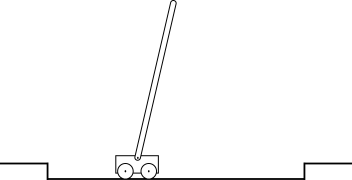
\includegraphics[scale=0.5]{14_rl/02_img/cartpole}
		\end{figure}
	}{0.39}{
		\begin{itemize}
			\item Move the cart \textbf{without} the pole falling over
			\item Action space $\mathcal{A}$:
			\begin{itemize}
				\item Move \textit{LEFT} (0)
				\item Move \textit{RIGHT} (1)
			\end{itemize}
			\item 4D state space $\mathcal{S}$:
			\begin{itemize}
				\item Cart position, velocity
				\item Angle of pole to cart...
				\item ...and its derivative
			\end{itemize}
		\end{itemize}
	}
\end{frame}


% Demo: Mountain Car Task
\begin{frame}{Demo: Mountain Car Task}{}
	\divideTwo{0.39}{
		\begin{itemize}
			\item The engine of the car is not strong enough
			\item You have to go back and forth to acquire momentum
			\item The car must not hit the wall (left side)
			\item The car has to reach the top of the hill
		\end{itemize}		
	}{0.60}{
		\begin{figure}
			\centering
			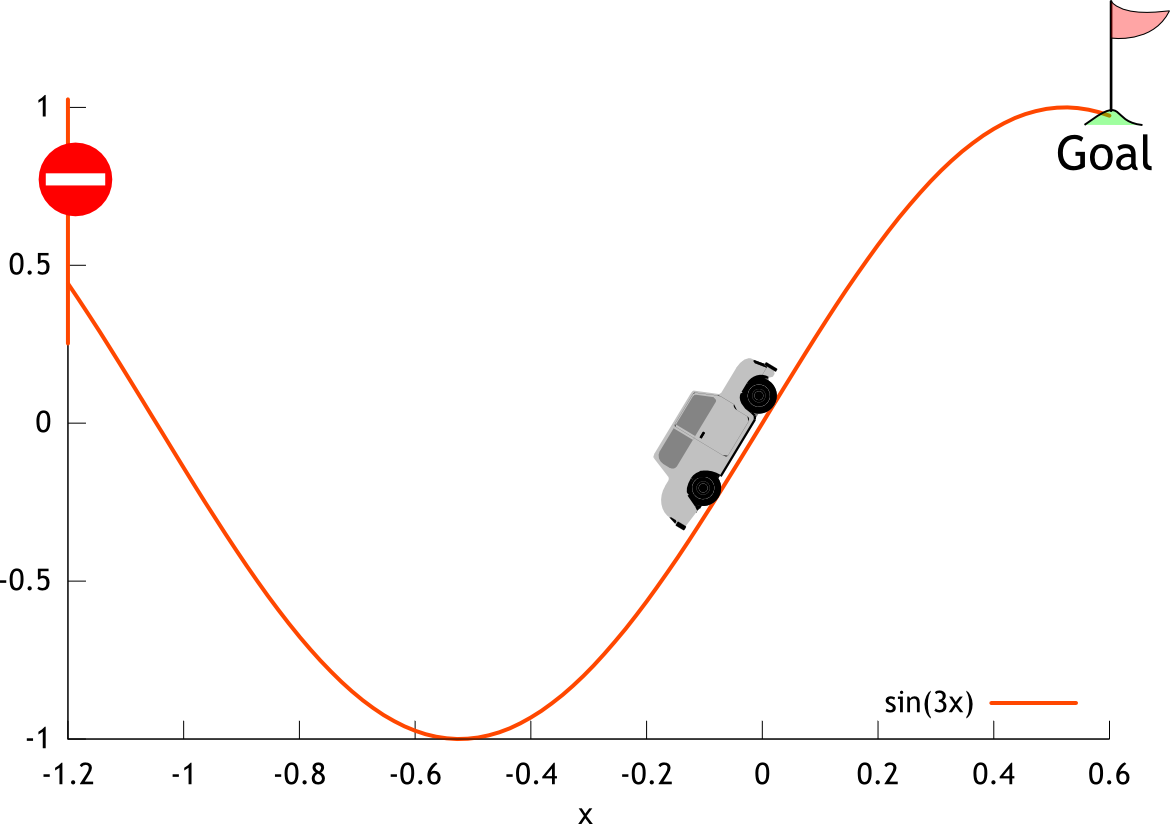
\includegraphics[scale=0.2]{14_rl/02_img/mountaincar}
		\end{figure}
	}
\end{frame}


% Demo: Taxi Task
\begin{frame}{Demo: Taxi Task}{}
	\divideTwo{0.49}{
		\begin{figure}
			\centering
			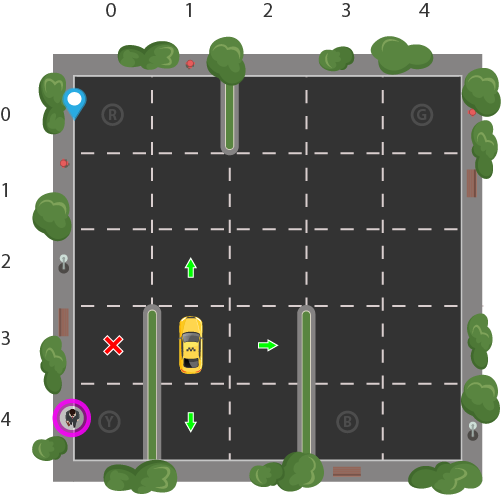
\includegraphics[scale=0.3]{14_rl/02_img/taxi}
		\end{figure}
	}{0.49}{
		\begin{itemize}
			\item Pick up passengers and get them to the drop-off location
			\item Filled square represents the taxi
			\item `|` represents a wall; you should not go there ;-)
			\item Blue letter: \textcolor{blue}{\textbf{Pick-up location}}
			\item Purple letter: \textcolor{violet}{\textbf{Drop-off location}}
			\item Taxi turns \textcolor{green}{\textbf{green}} if a passenger is aboard
		\end{itemize}
	}
\end{frame}


% Section: Advanced Algorithms
%______________________________________________________________________
\section{Advanced Algorithms}
\makedivider{Advanced Algorithms}

% Subsection: Policy Gradients Methods
% --------------------------------------------------------------------------------------------------------
\subsection{Policy Gradient Methods}


% Policy Gradient Methods
\begin{frame}{Policy Gradient Methods}{}
	\begin{itemize}
		\item Parameterize policy $\pi$ with parameters $\bm{\theta}$: $\pi_{\bm{\theta}}$
		\item Total reward for a trajectory $\tau$: $r(\tau)$
		\item \textbf{Goal:} Maximize the expected reward following a parameterized policy:
		\begin{equation}
			\mathcal{J}(\bm{\theta}) = \mathbb{E}_{\pi_{\bm{\theta}}} [r(\tau)]
		\end{equation}
		\item We can use gradient ascent to find the optimal parameters $\bm{\theta}^*$
		\item \Highlight{Problem:} How do we find the gradient of the objective which contains the expectation?
	\end{itemize}
\end{frame}


% Policy Gradient Theorem
\begin{frame}{Policy Gradient Theorem}{}
	\vspace*{-7mm}
	\begin{alignat*}{2}
		\nabla\mathbb{E}_{\pi_{\bm{\theta}}}
			&= \nabla\int \pi(\tau) r(\tau) \diff\tau						\\
			&= \int \nabla\pi(\tau) r(\tau) \diff\tau						
				&&\qquad\text{pull $\nabla$ inside} 					\\
			&= \int \pi(\tau) \nabla\log\pi(\tau) r(\tau) \diff\tau 			
				&&\qquad\text{use log trick: $\nabla_x \log(f(x)) = \frac{1}{f(x)}\nabla_x f(x)$}
															\\
			&= \mathbb{E}_{\pi_{\bm{\theta}}} [r(\tau) \nabla\log\pi(\tau)]
	\end{alignat*}
	\vspace*{-5mm}
	\hrule
	\vspace*{1mm}
	\begin{equation*}
		\pi_{\bm{\theta}}(\tau) = p(s_0) \cdot \prod_{t=1}^T \pi_{\bm{\theta}}(a_t \vert s_t) \cdot p(s_{t+1}, r_{t+1} \vert s_t, a_t)
	\end{equation*}
\end{frame}


% Policy Gradient Theorem
\begin{frame}{Policy Gradient Theorem}{}
	\begin{boxBlue}
		\highlight{Policy gradient theorem:} \\[2mm]
		\footnotesize
		\highlight{The derivative of the expected reward is the expectation of the product of the reward and gradient of the log of the policy $\pi_{\bm{\theta}}$.}
	\end{boxBlue}
\end{frame}


% Policy Gradient Theorem (Ctd.)
\begin{frame}{Policy Gradient Theorem (Ctd.)}{}
	\vspace*{-7mm}
	\begin{align*}
		\intertext{Taking the logarithm of $\pi_{\bm{\theta}}$, we get:}
		\log\pi_{\bm{\theta}}(\tau)
			&= \log p(s_0) + \sum_{t=1}^T \log \pi_{\bm{\theta}}(a_t \vert s_t) + \sum_{t=1}^T \log p(s_{t+1}, r_{t+1} \vert s_t, a_t) \\
		\nabla\log\pi_{\bm{\theta}}(\tau)
			&= \sum_{t=1}^T \nabla\log\pi_{\bm{\theta}}(a_t \vert s_t) \\
		\intertext{Putting it all together:}
		\Longrightarrow \nabla\mathbb{E}_{\pi_{\bm{\theta}}}[r(\tau)]
			&= \mathbb{E}_{\pi_{\bm{\theta}}}\left[ r(\tau) \cdot \left( \sum_{t=1}^T \nabla\log\pi_{\bm{\theta}}(a_t \vert s_t) \right) \right]
	\end{align*}
\end{frame}


% Policy Gradient Theorem (Ctd.)
\begin{frame}{Policy Gradient Theorem (Ctd.)}{}
	\begin{itemize}
		\item This result is appealing, since no knowledge about the initial state distribution nor the environment dynamics is necessary
		\item Therefore, this is an instance of a \highlight{model-free} algorithm
		\item There is still an expectation term in the equation, but we can sample a large number of trajectories and average \\
			$\Rightarrow$ \highlight{Markov Chain Monte Carlo (MCMC)}
		\item \Highlight{Problem: Reward term $r(\tau)$ adds a lot of variance to the sampling process}
			$\Rightarrow$ We can introduce a baseline
		\item Algorithm \highlight{REINFORCE}
	\end{itemize}
\end{frame}


% Subsection: Deep Reinforcement Learning
% --------------------------------------------------------------------------------------------------------
\subsection{Deep Reinforcement Learning}

% Deep Reinforcement Learning
\begin{frame}{Deep Reinforcement Learning}{}
	\begin{itemize}
		\item As already mentioned: The $Q$-learning table can become really large if the state space and the
			action space are really large
		\item \Highlight{It is not viable to maintain a table of all entries}
		\item Maybe it does not even fit into memory...
		\item An alternative is needed!
		\item \textbf{Idea}:
		\begin{itemize}
			\item Use deep learning methods to replace the table
			\item E.\,g. a deep MLP could predict the action to take
				given the observed state, the reward, ...
		\end{itemize}
	\end{itemize}
\end{frame}


% Deep Reinforcement Learning (Ctd.)
\begin{frame}{Deep Reinforcement Learning (Ctd.)}{}
	\begin{figure}
	\centering
	\begin{tikzpicture}[
		scale=0.4,
		every node/.style={scale=0.9}
	]
	
		\draw[very thick] (0,0) rectangle (15,10);
		\node at (2,9) {\textbf{Agent}};
		\draw[very thick] (18,0) rectangle (24,10);
		\node at (21,5) {\textbf{Environment}};

		\draw[very thick,->] (21,10) -- (21,12) -- node[below] {Reward} (7.5,12) -- (7.5,10);
		\draw[very thick,->] (21,0) -- (21,-2) -- node[above] {Observe state} (2,-2) -- (2,3.5);
		\draw[very thick,->] (14,3.9) -- node[above right=1mm and -4mm] {Action} (18,3.9);

		\node at (7.5,5) {
			\begin{tikzpicture}[scale=0.175]
				\draw[thick] (-10,1.5) rectangle (-5,7.5);
				\node at (-7.5,4.5) {State};
				\node at (5,14) {DNN};
				\node at (20,14) {$\pi_{\theta}(s, a)$};
				\node at (5,-6) {parameter $\theta$};

				% connections first layer to second layer
				\foreach \y in {-3,0,3,6,9,12}{\draw (0,\y) -- (-5,4.5);}

				% connections second layer to third layer
				\foreach \y in {-3,0,3,6,9,12}{\draw (0,\y) -- (10,-3);}
				\foreach \y in {-3,0,3,6,9,12}{\draw (0,\y) -- (10,0);}
				\foreach \y in {-3,0,3,6,9,12}{\draw (0,\y) -- (10,3);}
				\foreach \y in {-3,0,3,6,9,12}{\draw (0,\y) -- (10,6);}
				\foreach \y in {-3,0,3,6,9,12}{\draw (0,\y) -- (10,9);}
				\foreach \y in {-3,0,3,6,9,12}{\draw (0,\y) -- (10,12);}

				% connections third to fourth layer
				\foreach \y in {-3,0,3,6,9,12}{\draw (10,\y) -- (20,1.5);}
				\foreach \y in {-3,0,3,6,9,12}{\draw (10,\y) -- (20,4.5);}
				\foreach \y in {-3,0,3,6,9,12}{\draw (10,\y) -- (20,7.5);}

				% neurons
				\foreach \y in {-3,0,3,6,9,12}{\node[circle,draw=black,fill=myblue1] at (0,\y) {};}
				\foreach \y in {-3,0,3,6,9,12}{\node[circle,draw=black,fill=myblue1] at (10,\y) {};}
				\foreach \y in {1.5,4.5,7.5}{\node[circle,draw=black,double distance=1pt,fill=myblue1] at (20,\y) {};}
			\end{tikzpicture}
		};
		
	\end{tikzpicture}
\end{figure}
\end{frame}


% Deep Reinforcement Learning (Ctd.)
\begin{frame}[plain]{}{}
	\begin{figure}
		\centering
		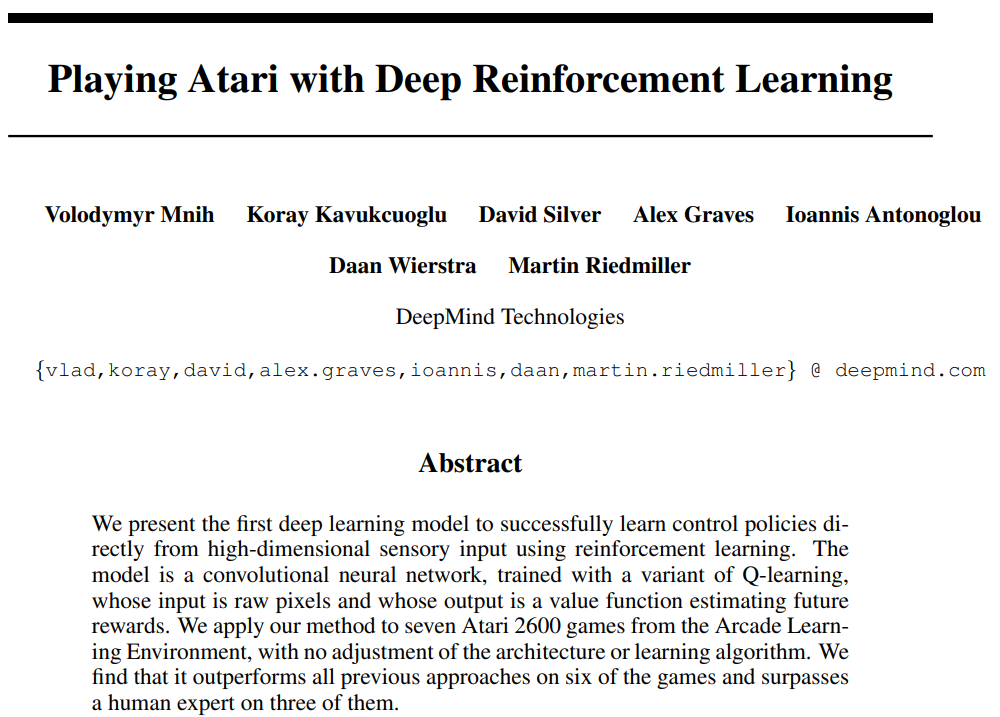
\includegraphics[scale=0.4]{14_rl/02_img/deep_q_learning_paper}
	\end{figure}
\end{frame}


% Section: Wrap-Up
%______________________________________________________________________
\section{Wrap-Up}
\makedivider{Wrap-Up}

% Subsection: Final Example
% --------------------------------------------------------------------------------------------------------
\subsection{Final Example}

% Final Example
\begin{frame}{Final Example}{}
	An agent can move in a simple deterministic world which looks as following:

	\begin{table}
		\centering
		\begin{tabular}{| c | c | c |}
			\hline
			\textbf{a} & \textbf{b} & \textbf{c} 		\\ \hline
			\textbf{d} & \textbf{e} & \highlight{f}		\\ \hline
		\end{tabular}
	\end{table}

	The agent can move up (u), down (d), left (l) or right (r), given the target field exists. The state `f' is an absorbing goal state. As soon as the agent reaches `f',
	it receives a reward of one point, otherwise 0 points. The discount factor $\gamma$ be set to 0.8.
\end{frame}


% Final Example (Ctd.)
\begin{frame}{Final Example -- Task a)}{}
	Specify the reward function $r(s, a)$ for all state-action pairs.
	
	\begin{table}
		\centering
		\begin{tabular}{| l | l | l | l | l |}
			\hline
			$r(a, r) = 0$ 	& 	$r(b, r) = 0$ 	& 	$r(c, d) = 1$ 	& $r(d, u) = 0$ 		& r(e, u) = 0		\\ \hline
			$r(a, d) = 0$ 	& 	$r(b, d) = 0$ 	& 	$r(c, l) = 0$ 	& $r(d, r) = 0$ 		& r(e, r) = 1		\\ \hline
			 			& 	$r(b, l) = 0$ 	&  				& 				& r(e, l) = 0		\\ \hline
		\end{tabular}
	\end{table}
\end{frame}


% Final Example (Ctd.)
\begin{frame}{Final Example -- Task b)}{}
	Calculate the value function $V^{\pi}(s)$ for all states $s$ given policy $\pi$:

	\begin{table}
		\centering
		\begin{tabular}{| c | c | c |}
			\hline
			$\rightarrow$ 	& 	$\rightarrow$ 	& 	$\downarrow$ 	\\ \hline
			$\uparrow$ 	& 	$\uparrow$ 	& 				\\ \hline
		\end{tabular}
	\end{table}

	\vspace*{-3mm}
	\begin{align*}
		V^{\pi}(d) 	&= \gamma^0 r(d, u) + \gamma^1 r(a, r) + \gamma^2 r(b, r) + \gamma^3 r(c,d) \\
					&= 1 \cdot 0 + 0.8 \cdot 0 + 0.8^2 \cdot 0 + 0.8^3 \cdot 1 = \bm{0.512}
	\end{align*}

	\vspace*{-4mm}
	\begin{table}
		\centering
		\begin{tabular}{| c | c | c |}
			\hline
			$V^{\pi}(a) = 0.640$		& 	$V^{\pi}(b) = 0.800$ 	&	$V^{\pi}(c) = 1.000$ 	\\ \hline
			$V^{\pi}(d) = 0.512$		&	$V^{\pi}(e) = 0.640$		&				\\ \hline
		\end{tabular}
	\end{table}
\end{frame}


% Final Example (Ctd.)
\begin{frame}{Final Example -- Task c)}{}
	How would \textbf{policy improvement} change the policy $\pi$ from task b) for state \textbf{e}? \\[5mm]

	Policy improvement: $\pi(s) = \argmax_{a \in \mathcal{A}} r(s, a) + \gamma V^{\pi}(\delta(s, a))$
	
	\begin{tabbing}
		\hspace*{1.5cm}\= \kill
		\textbf{up}:		\>	$0.64$ (cf. above) \\
		\textbf{left}: 		\>	$r(e, l) + \gamma V^{\pi}(d) = 0 + 0.8 \cdot 0.512 = 0.4096$ \\
		\textbf{right}: 		\>	$r(e, r) = 1$ \highlight{$\Longleftarrow$ We would take this one!}	
	\end{tabbing}

	$\Rightarrow \pi(\bm{e}) = right$
\end{frame}


% Final Example (Ctd.)
\begin{frame}{Final Example -- Task d)}{}
	Think of an optimal way to reach the goal state for each state $s$. Calculate $V^{\pi^*}(s)$. \\[5mm]
	
	Optimal routes: \\
	$a \longrightarrow b \longrightarrow c \longrightarrow f$ \\
	$a \longrightarrow d \longrightarrow e \longrightarrow f$

	\begin{table}
		\centering
		\begin{tabular}{| c | c | c |}
			\hline
			$V^{\pi^*}(a) = 0.640$		& 	$V^{\pi^*}(b) = 0.800$ 	&	$V^{\pi^*}(c) = 1.000$ 	\\ \hline
			$V^{\pi^*}(d) = 0.800$		&	$V^{\pi^*}(e) = 1.000$	&						\\ \hline
		\end{tabular}
	\end{table}
\end{frame}


% Final Example (Ctd.)
\begin{frame}{Final Example -- Task e)}{}
	Calculate the optimal $Q$-values for all possible state-action pairs. \\[5mm]
	
	\textbf{Hint:} Use the results from task d): $Q(s, a) = r(s, a) + \gamma V^{\pi^*}(s')$ \\[5mm]
	
	For state \textbf{a} we get: \\
	$Q(a, r) = r(a, r) + \gamma V^{\pi^*}(b) = 0 + 0.8 \cdot 0.8 = 0.64 = Q(a, u)$
	
	\begin{table}
		\centering
		\scalebox{0.8}{\begin{tabular}{| l | l | l | l | l |}
			\hline
			$Q(a, r) = 0.640$ 	& $Q(b, r) = 0.800$ 	& $Q(c, u) = 1.000$ 	& $Q(d, o) = 0.512$ 	& Q(e, o) = 0.640
			\\ \hline
			$Q(a, u) = 0.640$ 	& $Q(b, u) = 0.800$ 	& $Q(c, l) = 0.640$ 	& $Q(d, r) = 0.800$ 	& Q(e, r) = 1.000
			\\ \hline
			 				& $Q(b, l) = 0.512$ 	&  				& 				& Q(e, l) = 0.640	
			\\ \hline
		\end{tabular}}
	\end{table}
\end{frame}


% Subsection: Summary
% --------------------------------------------------------------------------------------------------------
\subsection{Summary}

% Summary
\begin{frame}{Summary}{}
	\begin{itemize}
		\item What is reinforcement learning?
		\begin{itemize}
			\item Learn optimal decisions based on feedback
			\item The agent only knows how good the action was, but not the optimal solution
			\item \highlight{Credit assignment problem}: \\
				Which move(s) is / are responsible for success / failure?
			\item Example: MENACE
		\end{itemize}
		\item Important terms:
		\begin{itemize}
			\item State $s$, action $a$
			\item Policy $\pi$ \textit{(optimal policy $\pi^*$)}
			\item Reward $r$ \textit{(immediate reward, discounted reward)}
		\end{itemize}
	\end{itemize}
\end{frame}


% Summary (Ctd.)
\begin{frame}{Summary (Ctd.)}{}
	\begin{itemize}
		\item Algorithms
		\begin{itemize}
			\item Policy iteration
			\item $Q$-learning
			\item SARSA
		\end{itemize}
		\item Exploitation vs. Exploration
		\begin{itemize}
			\item \highlight{Exploitation}: Exploit what is already known to be good
			\item \highlight{Exploration}: But don't miss to explore new states and actions
		\end{itemize}
		\item Non-deterministic case ($\delta(s, a)$ and $r(s, a)$ vary)
		\item Temporal difference learning
		\item Deep reinforcement learning
	\end{itemize}
\end{frame}


% Subsection: Recommended Literature and further Reading
% --------------------------------------------------------------------------------------------------------
\subsection{Recommended Literature and further Reading}

% Literature
%______________________________________________________________________
\begin{frame}[allowframebreaks]{Recommended Literature and further Reading}{}
	\footnotesize
	\begin{thebibliography}{2}
		\literature{book}{Mitchell.1997}{[1] Machine Learning}{T. Mitchell. McGraw-Hill Science. 1997.}
			{$\rightarrow$ \href{
				https://www.cs.ubbcluj.ro/~gabis/ml/ml-books/McGrawHill\%20-\%20Machine\%20Learning\%20-Tom\%20Mitchell.pdf
			}{\linkstyle{Click here}}, cf. chapter 13}
		\literature{online}{Valkov.2017}{[2] Solving an MDP with $Q$-Learning from scratch}{V. Valkov. 2017.}
			{$\rightarrow$
				\href{https://medium.com/@curiousily/solving-an-mdp-with-q-learning-from-scratch-deep-reinforcement-learning-for-hackers-part-1-45d1d360c120}{\linkstyle{Click here}}
			}
		\literature{book}{Geron.2017}{[3] Hands-On Machine Learning with Scikit-Learn \& TensorFlow}
			{A. Géron. O'Reilly. 2017.}
			{$\rightarrow$ \href{
				https://github.com/IsaacChanghau/DL-NLP-Readings/blob/master/Papers/Books/ML\%20DL\%20Coding/Python/Hands\%20on\%20Machine\%20Learning\%20with\%20Scikit\%20Learn\%20and\%20TensorFlow.pdf
			}{\linkstyle{Click here}}, cf. chapter 16}

		\literature{book}{Marsland.2015}{[4] Machine Learning; An algorithmic perspective}
			{S. Marsland. CRC Press. Chapman \& Hall. 2015.}
			{$\rightarrow$ \href{
				https://doc.lagout.org/science/Artificial\%20Intelligence/Machine\%20learning/Machine\%20Learning_\%20An\%20Algorithmic\%20Perspective\%20\%282nd\%20ed.\%29\%20\%5BMarsland\%202014-10-08\%5D.pdf
			}{\linkstyle{Click here}}, cf. chapter 17}

		\literature{article}{Sutton.1988}{[5] Learning to predict by the methods of temporal differences}
			{R. Sutton. Kluwer Academic Publishers. 1988.}
			{$\rightarrow$ \href{https://pdfs.semanticscholar.org/9c06/865e912788a6a51470724e087853d7269195.pdf}
			{\linkstyle{Click here}}}

		\literature{online}{Ng.2008}{[6] Machine Learning Lecture}
			{A. Ng. Stanford University. 2008.}
			{$\rightarrow$
				\href{https://www.youtube.com/watch?v=RtxI449ZjSc}
				{\linkstyle{Click here (Lecture 16)}},
				\href{https://www.youtube.com/watch?v=LKdFTsM3hl4&index=17&list=PLA89DCFA6ADACE599}
				{\linkstyle{Click here (Lecture 17)}},
				\href{https://www.youtube.com/watch?v=-ff6l5D8-j8&index=18&list=PLA89DCFA6ADACE599}
				{\linkstyle{Click here (Lecture 18)}},
				\href{https://www.youtube.com/watch?v=UFH5ibWnA7g&index=19&list=PLA89DCFA6ADACE599}
				{\linkstyle{Click here (Lecture 19)}},
				\href{https://www.youtube.com/watch?v=yCqPMD6coO8&list=PLA89DCFA6ADACE599&index=20}
				{\linkstyle{Click here (Lecture 20)}}
			}
			
		\literature{online}{AiGym}{[7] OpenAI Gym}{OpenAI. 2018.}
			{$\rightarrow$
				\href{https://gym.openai.com/}{\linkstyle{Click here}}
			}
			
		\literature{online}{Jaiswal.2017}{[8] Getting started with reinforcement Q-learning}
			{P. Jaiswal. Towards Data Science. 2017.}
			{$\rightarrow$
				\href{https://towardsdatascience.com/getting-started-with-reinforcement-q-learning-77499b1766b6}
				{\linkstyle{Click here}}
			}
		\literature{book}{Sutton.2014}{[9] Reinforcement Learning: An Introduction}{R. Sutton, A. Barto. MIT Press. 2014.}
			{$\rightarrow$ \href{
				http://incompleteideas.net/book/bookdraft2017nov5.pdf
			}{\linkstyle{Click here}}}
	\end{thebibliography}
\end{frame}


% Subsection: Meme of the Day
% --------------------------------------------------------------------------------------------------------
\subsection{Meme of the Day}

% Meme of the Day
\begin{frame}{Meme of the Day}{}
	\begin{figure}
		
\includegraphics[scale=0.30]{14_rl/02_img/meme_of_the_day}
	\end{figure}
\end{frame}


% Thank you
%______________________________________________________________________
\makethanks

\end{document}